%%% BEGIN EMBEDDED DATA (generated by tools/embed_data.sh, do not edit by hand)
%%% Regenerate with ./tools/embed_data.sh after re-running the benchmarks.
\begin{filecontents*}[overwrite]{csweep.dat}
c insavg lkavg case3 fallback case1 case2
0.2500 2.9391 242.8635 1406 5476 6786 0
0.5000 2.8929 166.1914 479 5446 7713 0
1.0000 2.9038 90.4372 0 5029 7778 414
2.0000 2.9092 115.5603 0 1985 4767 3425
4.0000 2.8911 163.0655 0 598 3402 4790
8.0000 2.9242 230.5490 0 140 2955 5237
16.0000 2.9198 285.6152 0 9 2825 5367
100.0000 2.9134 290.6818 0 0 2816 5376
\end{filecontents*}
\begin{filecontents*}[overwrite]{phivsmeasured.dat}
n meas3 phi3 meas8 phi8
4096 216.4 407.3 381.3 6829.9
8192 261.2 376.8 567.1 8941.5
16384 290.7 365.2 742.9 8785.3
32768 321.7 382.4 1073.2 8137.9
65536 352.1 384.7 1473.7 9873.4
131072 370.7 379.4 2055.7 9184.3
262144 375.4 377.5 2841.7 9111.1
1048576 377.3 378.3 4842.0 nan
\end{filecontents*}
\begin{filecontents*}[overwrite]{wl-elastic.dat}
load insavg insmax lkavg lkmax neg
87.500000 2.9208 92 345.3290 61092 787563
96.875000 4.2881 395 980.5294 318854 787563
99.218750 5.5726 701 1406.2222 282627 787563
99.609375 6.1741 801 1537.4680 350895 787563
\end{filecontents*}
\begin{filecontents*}[overwrite]{wl-funnel.dat}
load insavg insmax lkavg lkmax neg
87.500000 17.3970 61 17.3970 61 52
96.875000 33.2919 151 33.2919 151 147
99.218750 48.3263 295 48.3263 295 288
99.609375 56.2020 544 56.2020 544 545
\end{filecontents*}
\begin{filecontents*}[overwrite]{wl-standard.dat}
load insavg insmax lkavg lkmax neg
87.500000 4.2928 363 4.2928 363 14
96.875000 16.5016 4245 16.5016 4245 96
99.218750 45.9528 11519 45.9528 11519 1323
99.609375 61.9515 18585 61.9515 18585 1506
\end{filecontents*}
%%% END EMBEDDED DATA
% =====================================================================
%  Computer Engineering Project (PII) report
%  Elastic and Funnel Hashing: implementation and experimental evaluation
%  Michele Cioccarelli
%  Build with:  latexmk -pdf report.tex
% =====================================================================
\documentclass[11pt,a4paper]{article}

\usepackage[utf8]{inputenc}
\usepackage[T1]{fontenc}
\usepackage[english]{babel}
\usepackage{lmodern}
\usepackage{microtype}
\usepackage[a4paper,margin=2.6cm]{geometry}
\usepackage{amsmath,amssymb}
\usepackage{booktabs}
\usepackage{multirow}
\usepackage{array}
\usepackage{enumitem}
\usepackage{xcolor}
\usepackage{graphicx}
\usepackage{caption}
\usepackage{subcaption}
\usepackage{listings}
\usepackage{fancyhdr}
\usepackage{titlesec}
\usepackage{tikz}
\usepackage{pgfplots}
\usepackage[hidelinks]{hyperref}

\pgfplotsset{compat=1.18}
% The plot data is embedded at the top of this file and written out by filecontents at compile
% time, so the report is a single self-contained .tex with no external dependencies.
% Regenerate the embedded blocks with ./tools/embed_data.sh after re-running the benchmarks.
\usetikzlibrary{arrows.meta,positioning,fit,shapes.geometric,calc,backgrounds,decorations.pathreplacing}

\hypersetup{
    colorlinks=true,
    linkcolor=black,
    citecolor=black,
    urlcolor=blue!55!black,
    pdftitle={Elastic and Funnel Hashing: a C implementation and experimental evaluation},
    pdfauthor={Michele Cioccarelli}
}

% ---------------------------------------------------------------- style
\definecolor{codebg}{gray}{0.965}
\definecolor{rulec}{gray}{0.80}
\definecolor{accent}{HTML}{009689}
% Palette shared with the project slides: "twilight purple" for Elastic,
% "pastel sunset" for Funnel.
\definecolor{T1}{HTML}{9575CD}\definecolor{T2}{HTML}{B39DDB}
\definecolor{T3}{HTML}{D1C4E9}\definecolor{T4}{HTML}{C5CAE9}
\definecolor{T5}{HTML}{BBDEFB}
\definecolor{P1}{HTML}{D1C4E9}\definecolor{P2}{HTML}{F8BBD0}
\definecolor{P3}{HTML}{FFAB91}\definecolor{P4}{HTML}{FFCC80}
\definecolor{P5}{HTML}{FFE082}\definecolor{P6}{HTML}{FFF59D}
\definecolor{elasticc}{HTML}{9575CD}
\definecolor{funnelc}{HTML}{FFAB91}
\definecolor{stdc}{HTML}{466EB4}

\lstset{
    basicstyle=\ttfamily\footnotesize,
    backgroundcolor=\color{codebg},
    frame=single,
    rulecolor=\color{rulec},
    breaklines=true,
    columns=fullflexible,
    showstringspaces=false,
    xleftmargin=0.6em,
    xrightmargin=0.6em,
    aboveskip=0.9em,
    belowskip=0.9em,
}

\pagestyle{fancy}
\fancyhf{}
\lhead{\small Elastic and Funnel Hashing}
\rhead{\small Michele Cioccarelli}
\cfoot{\thepage}
\setlength{\headheight}{14pt}
\renewcommand{\headrulewidth}{0.4pt}

\titleformat{\section}{\large\bfseries\color{accent}}{\thesection.}{0.6em}{}
\titleformat{\subsection}{\normalsize\bfseries\boldmath}{\thesubsection.}{0.55em}{}
\titleformat{\subsubsection}{\small\bfseries\boldmath}{\thesubsubsection.}{0.5em}{}
\setlist[itemize]{leftmargin=1.4em,itemsep=0.22em,topsep=0.35em}
\setlist[enumerate]{leftmargin=1.7em,itemsep=0.28em,topsep=0.35em}

\captionsetup{font=small,labelfont=bf}

% Readability: the body was a wall of text. A small inter-paragraph skip separates the
% paragraphs visually and costs nothing in page count; opening the leading as well would look
% marginally better but adds two pages, so it is left alone.
\setlength{\parskip}{0.45em}
\setlength{\parindent}{1.2em}

% shorthand
\newcommand{\dinv}{\delta^{-1}}
\newcommand{\Ai}{A_i}
\newcommand{\phimap}{\varphi}
\newcommand{\code}[1]{\texttt{\small #1}}

\begin{document}

% =====================================================================
\begin{titlepage}
\centering
\vspace*{1.5cm}
{\large POLITECNICO DI MILANO}\\[0.3cm]
{\normalsize Department of Electronics, Information and Bioengineering}\\[0.2cm]
{\normalsize Computer Engineering Project (PII), A.Y. 2025/26}\\[2.4cm]

{\Huge\bfseries Elastic and Funnel Hashing\par}
\vspace{0.5cm}
{\LARGE A C implementation and experimental evaluation\par}
\vspace{0.45cm}
{\large\itshape after Farach-Colton, Krapivin and Kuszmaul,\\
``Optimal Bounds for Open Addressing Without Reordering'' (2025)\par}

\vspace{2.6cm}
\begin{tabular}{rl}
\textbf{Author} & Michele Cioccarelli\\[0.35em]
\textbf{Supervisor} & Prof. Alessandro Barenghi\\[0.35em]
\textbf{Course owner} & Prof. Mariagrazia Fugini\\[0.35em]
\textbf{Duration} & November 2025 -- September 2026\\
\end{tabular}

\vspace{0.9cm}
{\small Paper: \url{https://arxiv.org/abs/2501.02305}\\[0.25em]
Repository: \url{https://github.com/MicheleCioccarelli/Hashmap_benchmarking}}

\vfill
\end{titlepage}

\pagenumbering{roman}
\tableofcontents
\newpage
\pagenumbering{arabic}

% =====================================================================
\section{Introduction}
% =====================================================================

\subsection{Context}
\label{sec:context}

This project is a faithful implementation and benchmarking of the data structures presented in the paper by Farach-Colton, Krapivin and Kuszmaul, \emph{Optimal Bounds for Open Addressing
Without Reordering} \cite{paper}.

An \emph{open-addressed} hash table stores every key directly in a slot of an array of
size $n$.
This data structure is based on a hash function $h_i(x)$, which takes an element $x$ as an argument and returns a memory slot for the $i$-th insertion/search attempt.
A call to the hash function is called a \emph{probe}.

Each key $x$ has a \emph{probe sequence}
$h_1(x), h_2(x), \dots$ which is the succession of slots that subsequent calls to the hash functions will yield

The quantity governing the behavior of the structure is the free-space fraction
\[
    \delta \;=\; 1 - \text{load factor}
\]
that is, the share of slots left empty after inserting $n - \lfloor \delta n \rfloor$ keys, or more simply it describes \emph{how much} of the table is free at a specific time.
It is interesting to observe the behavior of data structures when $\delta$ approaches $0$.

The rest of the report uses this notation throughout:

\begin{center}
\small
\renewcommand{\arraystretch}{1.45}
\begin{tabular}{@{}l@{\hspace{2.2em}}l@{}}
\toprule
$A$ & the single physical array holding the table, of size $n$ \\
$n$ & the capacity of $A$, in slots \\
$x$ & a key; the tables in this project store strings \\
$h_k(x)$ & the slot proposed by the $k$-th probe for $x$ \\
$\delta$ & the free-space fraction, so $n - \lfloor \delta n \rfloor$ keys are inserted \\
positive query & a search for a key that is in the table \\
negative query & a search for a key that is not in the table \\
\bottomrule
\end{tabular}
\end{center}

It was historically believed that \emph{uniform probing} was optimal. In this scheme, the probe sequence is a truly random permutation
of $\{1,\dots,n\}$ and each insertion greedily takes the first free slot it finds. Its
amortized expected probe complexity is $\Theta(\log \dinv)$. 

Ullman \cite{ullman1972} conjectured in 1972 that this was
optimal for every \emph{greedy} algorithm. Later Yao proved it in 1985 in the paper
\emph{Uniform Hashing is Optimal} \cite{yao1985}. In the same work Yao stated a stronger conjecture: that
any greedy table must have \emph{worst-case} expected probe complexity at least $(1-o(1))\dinv$.

For a long time it was believed that beating these bounds wasn't possible, so the way people got around them was by relaxing the problem by allowing
\emph{reordering} of already inserted elements.

The paper examined in this work was the first to break Yao's conjecture by introducing two schemes that never reorder an element and that beat both expected bounds:

\begin{itemize}
  \item \emph{Elastic Hashing}, non-greedy, with $O(1)$ amortized expected search cost and
        $O(\log \dinv)$ worst-case expected cost;
  \item \emph{Funnel Hashing}, greedy, with $O(\log^2 \dinv)$ worst-case expected cost,
        which is $o(\dinv)$ and therefore \emph{disproves Yao's conjecture}.
\end{itemize}

Both results come with matching lower bounds, so the schemes are asymptotically optimal in
their respective classes.

\subsection{Goal of the project}

The paper is a purely theoretical work: it proves asymptotic bounds but provides no
implementation, fixes no constants, and leaves several operational points open. The goal of
this project is to close that gap:

\begin{itemize}
  \item implement Elastic Hashing and Funnel Hashing as real hash tables in C,
        working on string keys for easy benchmarking;
  \item resolve the points the paper leaves unspecified but which become mandatory
        in a concrete implementation, in particular a search algorithm for
        Elastic Hashing, the constant $c$, and the cost of negative queries, which the paper bounds
        only for greedy schemes and leaves open for Elastic Hashing;
  \item measure the behavior of the two structures at concrete, finite values of $n$ and
        $\delta$ against a linear-probing
        control table, with exact probe counting instrumentation;
  \item document the distance between the theoretical model and what is actually
        observed at concrete values of $n$ and $\delta$, along with potential hidden constants.
\end{itemize}

Of these, the second is where most of the original work went, and
Section~\ref{sec:lookup-elastic} is devoted to it.

\subsection{Project information}

\begin{center}
\begin{tabular}{@{}>{\bfseries}lp{0.66\linewidth}@{}}
\toprule
Title & Elastic and Funnel Hashing: a C implementation and experimental evaluation \\
Author & Michele Cioccarelli \\
Supervisor & Prof. Alessandro Barenghi \\
Reference paper & Farach-Colton, Krapivin, Kuszmaul, \emph{Optimal Bounds for Open
Addressing Without Reordering}, arXiv:2501.02305 \\
Implementation & C11, 4,253 lines of sources and headers, plus 5,840 lines of tests \\
Repository & \url{https://github.com/MicheleCioccarelli/Hashmap_benchmarking} \\
\bottomrule
\end{tabular}
\end{center}

\subsection{Timeline}

The project ran over three distinct phases: study of the paper and of its proofs from
November 2025 to February 2026, preparation of a detailed presentation of its results from
February to May 2026, and implementation, instrumentation and experimental benchmarking from
July to September 2026. The long study phase was necessary because this is a very dense
paper.

\section{Related work}
\label{sec:related}

Open addressing without reordering has a long and well-delimited history. Knuth analyzed
linear probing in 1963 \cite{knuth1963,knuth1998}, obtaining an expected insertion time of
$O(\delta^{-2})$ and an amortized expected probe complexity of $O(\dinv)$. Ullman conjectured
in 1972 that $\Theta(\log\dinv)$ amortized was optimal for every greedy algorithm
\cite{ullman1972}, and Yao proved it in 1985 \cite{yao1985}, conjecturing at the same time
that the worst-case expected probe complexity of a greedy table could not fall below
$\Omega(\dinv)$. 

The classical way around these bounds was to relax the problem and permit
\emph{reordering} of inserted elements, under which $O(1)$ amortized is reachable even for a
full table \cite{brent1973,gonnet1979}. More recently, tiny pointers showed that allowing
deletions as well as insertions pushes the optimal cost to $\delta^{-\Omega(1)}$
\cite{tinypointers}. The paper implemented here \cite{paper} is what disproves Yao's
conjecture without reordering, with matching lower bounds for both of its schemes.

Since the paper was published, several independent implementations
of the two schemes have been published: Python packages \cite{optopenhash,jorgik}, Go
\cite{karpeles,bdragon} and C++ \cite{ascv}. This project is therefore not the first
implementation. It differs from the existing ones in two
respects, both of which concern \emph{what is measured} rather than the algorithms
themselves.

\begin{enumerate}
  \item The measured quantity: the published benchmarks we could inspect compare
        wall-clock time against the language's built-in hash map \cite{karpeles}. That is a
        legitimate engineering question, but it is not the quantity the paper's theorems are
        stated over. This project measures \emph{probe counts} as a function of the load
        factor, which is the quantity that appears in Theorems 1 and 2 and is independent of
        machine and language.
  \item The definition of search cost: the paper's model charges a search for the
        position of the key in the single flat sequence a query walks from the beginning. The
        most widely referenced Python implementation \cite{optopenhash} searches a different
        way: by walking the two-dimensional structure the insertion used, level by level. Both
        find the key, but they count different things, and only the first is the quantity the
        theorems bound. Section~\ref{sec:ijscan} explains why the difference matters and what it
        costs.
\end{enumerate}

All the
implementations cited above provide Funnel Hashing as well as Elastic Hashing, and they agree with
this project on the outer structure: $\alpha = \lceil 4\log_2\dinv\rceil + 10$,
$\beta = \lceil 2\log_2\dinv\rceil$, levels subdivided into buckets of $\beta$ slots, and one
bucket scanned per level. They differ on the two points where the paper is most demanding.

\begin{itemize}
  \item The special array: the paper splits $A_{\alpha+1}$ into a uniform table $B$,
        capped at $\log\log n$ attempts, and a \emph{two-choice} table $C$ with buckets of
        $2\log\log n$ slots, and it is $C$ that delivers the high-probability worst-case
        bound through the power-of-two-choices theorem. The most referenced Python
        implementation \cite{optopenhash} instead probes the special array with \\
        \code{idx = (hash(key) + j) \% size}, that is \emph{linear probing} capped at
        $\lceil\log\log n\rceil$ attempts, with a two-index fallback. It is a simpler and
        perfectly workable structure, but it is not the construction the worst-case bound is
        proved about. This project implements $B$ and $C$ as described.
  \item The level sizes: the same implementation sets
        \code{a\_i = max(1, round(a1 * 0.75**i))}, a direct rounding of a real geometric
        sequence. That does satisfy $a_{i+1} = 3a_i/4 \pm 1$, but the terms do not sum exactly
        to $|A'|/\beta$, so the levels do not tile $A'$ exactly. This project chooses the
        sequence so that both hold at once.
\end{itemize}

We found no published study of the \emph{finite} behavior of the two schemes: the paper is
recent and its results are asymptotic, and we could find no measurement of the size of the
constants hidden inside the $O(\cdot)$ notation. That gap is what
Section~\ref{sec:results} attempts to fill.

\newpage

\section{Innovation introduced}
\label{sec:innovation}

The contribution of this project is implementational and experimental, and has three parts.

\begin{enumerate}
  \item A search algorithm for Elastic Hashing: the paper states the identity that
        links insertion to search, but never turns it into a procedure a query can run, and
        leaves part of the probe sequence undefined. This project derives one, validates it
        experimentally, and shows it reproduces the sequence the insertion actually used,
        which is what makes the measured cost the quantity the theorem bounds
        (Section~\ref{sec:lookup-elastic}).
  \item A value for the constant $c$: the paper asks only that $c$ be
        ``sufficiently large''. It turns out not to be a neutral choice at finite sizes: it
        moves search cost by more than a factor of 3 and controls how often the expensive
        insertion case occurs (Section~\ref{sec:results-c}).
  \item The distance between asymptotic and measured: at $n = 65{,}536$ the
        insertion advantage of Elastic Hashing is plainly visible, while its search advantage
        is entirely hidden by a large constant. Section~\ref{sec:results-bounds} compares each
        measured average against the shape its theorem predicts. This cannot be read off the
        paper, which reasons up to constants.
\end{enumerate}

\section{The hashing schemes}
\label{sec:algorithms}

This section describes what the two hash tables actually do, then Section~\ref{sec:implementation}
turns to how they were implemented and to the questions the paper leaves open.
Lemmas and theorems are cited by number where they are used, and are stated without
proof: the proofs are in the original paper \cite{paper}, and reproducing them here would not
help a reader who wants to know what the structures do.

\subsection{Cost model and metrics}

Recall the probe sequence $h_1(x), h_2(x), \dots$ of Section~\ref{sec:context}. Two things need adding
to it before the metrics can be stated. The sequence is drawn from a distribution
$\mathcal{P}$, and an insertion must place $x$ in some $h_j(x)$ that is free at that moment,
also it may not
move keys already inserted. That prohibition is what the word \emph{reordering} refers to
throughout.

If $x$ is placed in $h_k(x)$, then $x$ has \emph{probe complexity} $k$: a query needs to
inspect exactly the first $k$ entries of $x$'s sequence to reach it. This single number is
what every bound in the paper is stated over, and it is also what this project measures.

In practice we measure a \emph{probe} as the inspection of one physical slot of the table.

The following do \emph{not} count as probes: hash computation, partition construction,
string comparisons and temporary allocations. Repeatedly generated positions count
repeatedly, because the model samples \emph{with replacement}: if the hash function proposes
the same slot twice, that is the cost the algorithm actually pays.

\subsubsection{Metrics}

These are the metrics by which we measure hashing performance. The table below collects, for each of the three structures, the bound claimed for it in each metric.

All three are built from the same per-key number, the probe complexity of $x$ defined
above. They differ only in the order in which the average over keys and the expectation over
the random hash draws are taken, and that order is what makes them hard or easy to satisfy.

\begin{description}[leftmargin=0em,style=nextline]
  \item[Amortized expected probe complexity]
        This is the expected value of the \emph{average} probe complexity taken over all the inserted
        keys. Very low bounds are reachable here even when individual keys are expensive,
        because the probing cost of an unlucky key is spread across all the others.
        Average first, then expectation.

  \item[Worst-case expected probe complexity]
        Take each key on its own and compute the expected value of \emph{its} probe
        complexity; this metric is the largest of those values, over all the keys inserted.
        Expectation first, then maximum. It is not an average over the keys and it is not
        amortized: an unlucky key can no longer be paid for by the cheap ones, which is why
        the bound is much harder to achieve and why Yao conjectured it could not be pushed
        below $\Omega(\dinv)$.
  \item[High-probability worst case]
        Here there is no expectation at all. This is a value that the most expensive key
        of an entire run stays below with probability $1 - 1/\mathrm{poly}(n)$, that is, in
        all runs except a vanishing fraction. Only Funnel Hashing is given such a bound.
\end{description}

\begin{center}
\small
\begin{tabular}{@{}lccc@{}}
\toprule
\textbf{Probe complexity} & \textbf{Control} & \textbf{Elastic} & \textbf{Funnel} \\
 & \emph{linear probing} & Theorem 1 & Theorem 2 \\
\midrule
Amortized expected & $\Theta(\dinv)$ & $O(1)$ & $O(\log\dinv)$ \\
Worst-case expected & $\Theta(\delta^{-2})$ & $O(\log\dinv)$ & $O(\log^2\dinv)$ \\
Worst case, high probability & --- & --- & $O(\log^2\dinv + \log\log n)$ \\
\bottomrule
\end{tabular}
\end{center}

The Control column does not come from the paper. Both entries are classical results on linear
probing due to Knuth \cite{knuth1963,knuth1998}: the amortized expected probe complexity is
$\Theta(\dinv)$, and the expected cost of an insertion into a table already at load
$1 - \delta$ is $\Theta(\delta^{-2})$. The second entry is the first result read through the
report's own definitions rather than a statement quoted from Knuth: linear probing is greedy,
so a key's probe complexity equals the number of probes its insertion made, and the largest of
those expectations is the one belonging to the last key inserted. 

A dash means the source states no
bound of that kind, not that the quantity is unbounded: only Funnel Hashing is given a
high-probability guarantee.

Note that the maximum observed in a single run is not the worst-case expected quantity: it is
one realization of a random variable, not an expectation. Maxima are reported below as a
diagnostic of the tail, not as verification of a bound.
\subsection{Elastic Hashing}
\label{sec:elastic}

This is a \emph{non-greedy} open addressing hashing scheme. At a high level, it works by dividing the main array $A$ (of size $n$) into $\log(n)$ subarrays and picking very convenient insertion slots.

\subsubsection{Partitioning the table}

First, $A$ is split into $\lceil \log_2 n \rceil$ contiguous subarrays
$A_1, A_2, \dots$ of geometrically decreasing length:
\[
    |A_{i+1}| = |A_i| / 2 \pm 1 ,
\]
where the $\pm 1$ exists so that the sum $\sum_i |A_i| = n$ doesn't break for arbitrary
capacities.

\subsubsection{The function \texorpdfstring{$\phimap$}{phi}}
This is the main idea behind elastic hashing, it is also the harder to understand.

Classical open addressing gives a key $x$ one flat
sequence of candidate slots $h_1(x), h_2(x), \dots$. A key placed in $h_7(x)$ costs 7 probes.

This insertion algorithm does not address probes
that way. Since $A$ is split into subarrays, a probe is a choice of subarray together with an
attempt inside it, so it takes two indices: $h_{i,j}(x)$ denotes the $j$-th attempt in $A_i$.
Figure~\ref{fig:phi2d} shows this grid.

These two notations are reconciled by an injection
$\phimap : \mathbb{Z}^+ \times \mathbb{Z}^+ \to \mathbb{Z}^+$, which numbers the cells of the
grid, together with the definition
\[
    h_{\phimap(i,j)}(x) \;:=\; h_{i,j}(x) .
\]
A key placed at $(i,j)$ therefore has probe complexity $\phimap(i,j)$. Injectivity is what
makes the definition consistent: no two cells claim the same position of the flat sequence.

More details on how $\phimap$ is constructed are available in the original paper.

What $\phimap$ actually means is an upper bound on search probe complexity, which in
non-greedy open addressing is a different quantity from insertion probe complexity.

\begin{quote}
If the insertion placed $x$ at local coordinate $(i,j)$, then $\phimap(i,j)$ is a
\emph{hard upper bound} on the number of probes a search for $x$ can ever need. A present
key is guaranteed to be found at or before global probe $\phimap(i,j)$.
\end{quote}

This means that the real objective of the insertion algorithm is picking spots which
minimize $\phimap$, in order to allow fast lookup times.

Two practical consequences follow, and both are visible in the measurements later:

\begin{itemize}
  \item \emph{Making many attempts inside the same subarray is very expensive in search
        terms}, because $\phimap$ grows quadratically in $j$, whereas changing subarray costs only
        linearly in $i$. The algorithm is built to exploit this asymmetry, which is why Case 1 gives up
        on $A_i$ after $f(\varepsilon)$ attempts and falls back to $A_{i+1}$.
  \item The search cost of a key is the integer $\phimap(i,j)$ itself, not a quantity
        proportional to it. This is unusual, and it is what makes the encoding matter in
        practice rather than only asymptotically. Take the cell highlighted in
        Figure~\ref{fig:phi2d}: a key found at $(2,2)$ was placed on the second attempt in the
        second subarray, which is close to the best outcome the algorithm can produce, and yet
        it costs $\phimap(2,2) = 114$ probes to retrieve. Even the very best possible
        placement, $(1,1)$, costs 13. The bound $\phimap(i,j) \le O(i j^2)$ is not violated by
        this: the multiplicative constant inside the $O(\cdot)$ is simply large, and at the
        capacities measured here it is that constant, and not the growth rate, that determines
        what a search actually pays (Section~\ref{sec:results-lookup}).
\end{itemize}

\begin{center}
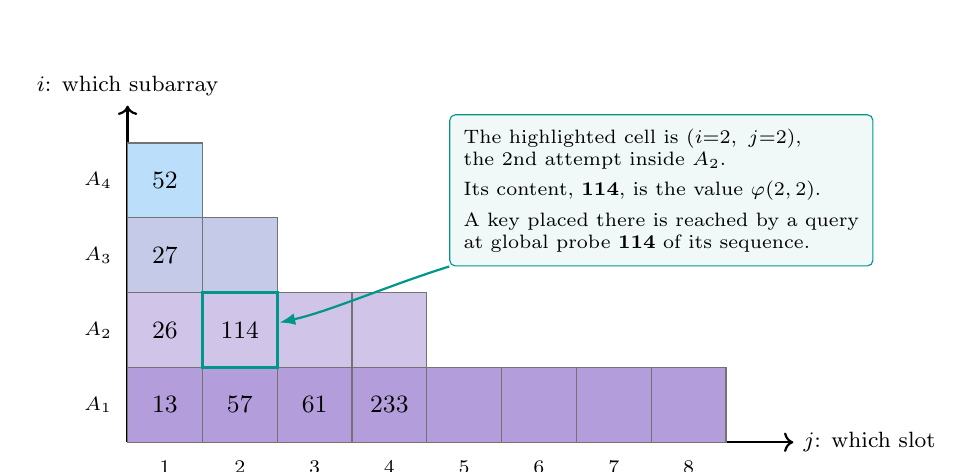
\begin{tikzpicture}[scale=0.95,every node/.style={font=\small}]
  % axes
  \draw[->,thick] (0,0) -- (8.9,0) node[right,font=\footnotesize] {$j$: which slot};
  \draw[->,thick] (0,0) -- (0,4.5) node[above,font=\footnotesize] {$i$: which subarray};
  \foreach \j in {1,...,8} \node[font=\scriptsize] at (\j-0.5,-0.33) {\j};
  \foreach \i/\lab in {1/$A_1$,2/$A_2$,3/$A_3$,4/$A_4$}
     \node[font=\scriptsize,left] at (-0.08,\i-0.5) {\lab};
  % cells
  \foreach \j in {1,...,8} \fill[T2,draw=black!55] (\j-1,0) rectangle (\j,1);
  \foreach \j in {1,...,4} \fill[T3,draw=black!55] (\j-1,1) rectangle (\j,2);
  \foreach \j in {1,...,2} \fill[T4,draw=black!55] (\j-1,2) rectangle (\j,3);
  \fill[T5,draw=black!55] (0,3) rectangle (1,4);
  % values
  \node at (0.5,0.5) {13};   \node at (1.5,0.5) {57};
  \node at (2.5,0.5) {61};   \node at (3.5,0.5) {233};
  \node at (0.5,1.5) {26};   \node at (1.5,1.5) {114};
  \node at (0.5,2.5) {27};   \node at (0.5,3.5) {52};
  % callout on one specific cell, placed in the empty upper-right region
  \draw[very thick,accent] (1,1) rectangle (2,2);
  \node[anchor=south west,align=left,font=\scriptsize,draw=accent,rounded corners=2pt,
        fill=accent!6,inner sep=5pt] (callout) at (4.3,2.35)
       {The highlighted cell is $(i{=}2,\ j{=}2)$,\\
        the 2nd attempt inside $A_2$.\\[3pt]
        Its content, \textbf{114}, is the value $\varphi(2,2)$.\\[3pt]
        A key placed there is reached by a query\\
        at global probe \textbf{114} of its sequence.};
  \draw[accent,thick,-{Latex[length=2mm]}] (callout.south west) .. controls (3.5,2.1) and (2.7,1.75) .. (2.03,1.6);
\end{tikzpicture}
\end{center}
{\captionof{figure}{Two-dimensional probing structure. The number written inside each
cell is the value of $\phimap(i,j)$ for that cell, computed by the implementation, that is,
the position in the one-dimensional sequence at which a key placed there will be found. Note the rapid growth along $j$
($13 \to 57 \to 61 \to 233$) compared with the growth along $i$ ($13 \to 26 \to 27$): this
asymmetry is what the algorithm exploits, and it is also the reason for the high finite
search costs measured in Section~\ref{sec:results-lookup}.}
\label{fig:phi2d}\par}

\subsubsection{Insertion batches}

The $n - \lfloor \delta n \rfloor$ insertions are divided into \emph{batches}
$\mathcal{B}_0, \mathcal{B}_1, \dots$. 
Each batch $\mathcal{B}_i$ inserts element into arrays $A_i, A_{i+1}$. 

At the end of each batch this invariant must be true: every $A_j$ with
$j \le i$ contains exactly $|A_j| - \lfloor \delta|A_j|/2 \rfloor$ elements and $A_{i+1}$
contains exactly $\lceil 0.75 |A_{i+1}| \rceil$, The only exception is $\mathcal{B}_0$, which fills $A_1$ up to $\lceil 0.75\,|A_1| \rceil$ elements greedily.

Each subsequent batch $\mathcal{B}_i$  performs
$
    |A_i| - \lfloor \delta |A_i| / 2 \rfloor - \lceil 0.75\,|A_i| \rceil
    + \lceil 0.75\,|A_{i+1}| \rceil
$ insertions

 
 Since batch sizes decrease geometrically,
the whole sequence finishes within $O(\log \dinv)$ batches.

Each batch $\mathcal{B}_i$ with $i\neq0$ handles insertions based on how full $A_i$ and $A_{i+1}$ are. For brevity we define $\epsilon_i$ as the free fraction of $A_i$ (its local $\delta$)

We also need to define
\[
    f(\epsilon) \;=\; c \cdot \min\!\left( \log^2 \varepsilon^{-1},\; \log \dinv \right),
\]

This is a hard limit on how many probes should be done in a particular subarray before it becomes very inefficient.

Every insertion falls into one of three
cases.

\begin{center}
\small
\renewcommand{\arraystretch}{1.55}
\begin{tabular}{@{}clp{0.50\linewidth}@{}}
\toprule
\textbf{Case} & \textbf{Condition} & \textbf{Action} \\
\midrule
1 & $\epsilon_i > \delta/2$ and $\epsilon_{i+1} > 0.25$ &
Try at most $f(\epsilon_i)$ positions in $A_i$; if all fail, fall back to the first free
slot of $A_{i+1}$. \\[0.35em]
2 & $\epsilon_i \le \delta/2$ &
$A_i$ is too full: the key goes to the first free slot of $A_{i+1}$. \\[0.35em]
3 & $\epsilon_{i+1} \le 0.25$ &
$A_{i+1}$ is too full: the key goes to the first free slot of $A_i$, with uniform probing
over a potentially saturated array. \\
\bottomrule
\end{tabular}
\end{center}

Case 3 is the \emph{expensive case}. Lemma 2 of the paper guarantees that with probability
at least $1 - O(1/|A_i|^2)$ no insertion of batch $\mathcal{B}_i$ falls into it;
Section~\ref{sec:results-c} measures how often Case 3 actually fires as $c$ is varied.

\subsection{Funnel Hashing}
\label{sec:funnel}

Funnel Hashing is conceptually simpler than Elastic Hashing because it stays \emph{greedy}: every
key must take the first free slot of its sequence. The gain over uniform probing comes not from
abandoning greediness, but from the \emph{shape} of the sequence.

The layout prescribed by this hashing scheme is quite complex, we will refer to an \emph{array of arrays} as simply array, and an \emph{array of keys} as a bucket

\subsubsection{Parameters and partition}

Assuming without loss of generality that $\delta \le 1/8$, one defines
\[
    \alpha = \lceil 4 \log_2 \dinv \rceil + 10 ,
    \qquad
    \beta  = \lceil 2 \log_2 \dinv \rceil 
\]

The main array $A$ is split into $A'$, where the vast majority of insertions happen, and a special
array $A_{\alpha+1}$, with
\[
    \lfloor 3\delta n/4 \rfloor \;\ge\; |A_{\alpha+1}| \;\ge\; \lceil \delta n/2 \rceil
\]
this layout allows $|A'|$ to be divisible by $\beta$. 

In turn $A'$ is split into
$\alpha$ subarrays $A_1,\dots,A_\alpha$ with $|A_i| = \beta a_i$, where $a_i$ is the number
of \emph{buckets} of $\beta$ slots each and
\[
    a_{i+1} = 3a_i/4 \pm 1 .
\]

\begin{center}
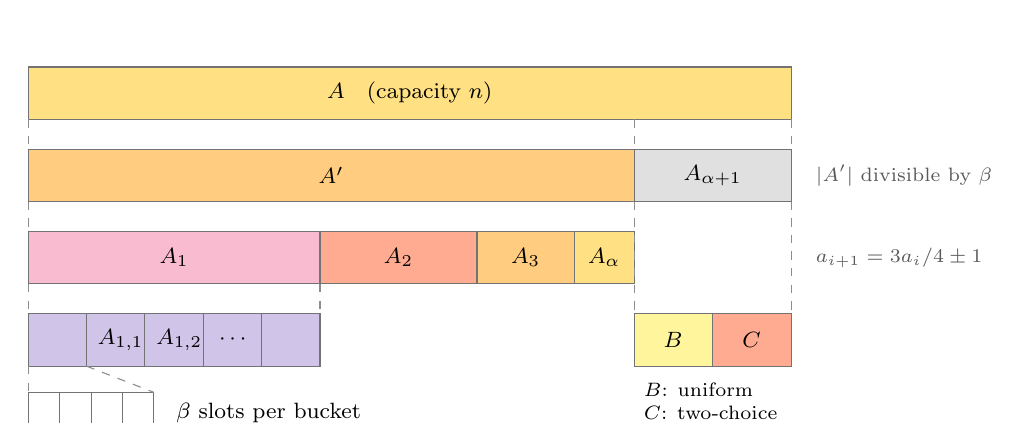
\begin{tikzpicture}[scale=0.95,every node/.style={font=\footnotesize}]
  % level A
  \draw[fill=P5,draw=black!55] (0,4.2) rectangle (10.2,4.9);
  \node at (5.1,4.55) {$A$ \; (capacity $n$)};
  % level A' / A_alpha+1
  \draw[fill=P4,draw=black!55] (0,3.1) rectangle (8.1,3.8);
  \node at (4.05,3.45) {$A'$};
  \draw[fill=black!12,draw=black!55] (8.1,3.1) rectangle (10.2,3.8);
  \node at (9.15,3.45) {$A_{\alpha+1}$};
  \draw[dashed,black!45] (0,4.2)--(0,3.8); \draw[dashed,black!45] (8.1,4.2)--(8.1,3.8);
  \draw[dashed,black!45] (10.2,4.2)--(10.2,3.8);
  % level Ai
  \draw[fill=P2,draw=black!55] (0,2.0) rectangle (3.9,2.7); \node at (1.95,2.35) {$A_1$};
  \draw[fill=P3,draw=black!55] (3.9,2.0) rectangle (6.0,2.7); \node at (4.95,2.35) {$A_2$};
  \draw[fill=P4,draw=black!55] (6.0,2.0) rectangle (7.3,2.7); \node at (6.65,2.35) {$A_3$};
  \draw[fill=P5,draw=black!55] (7.3,2.0) rectangle (8.1,2.7); \node at (7.7,2.35) {$A_\alpha$};
  \draw[dashed,black!45] (0,3.1)--(0,2.7); \draw[dashed,black!45] (8.1,3.1)--(8.1,2.7);
  % buckets of A1
  \foreach \x in {0,1,...,4} {
     \draw[fill=P1,draw=black!55] (\x*0.78,0.9) rectangle (\x*0.78+0.78,1.6);
  }
  \node at (1.95,1.25) {$A_{1,1} \;\; A_{1,2} \;\; \cdots$};
  \draw[dashed,black!45] (0,2.0)--(0,1.6); \draw[dashed,black!45] (3.9,2.0)--(3.9,1.6);
  % slots
  \foreach \x in {0,1,2,3} \draw[fill=white,draw=black!55] (\x*0.42,0) rectangle (\x*0.42+0.42,0.55);
  \node[right] at (1.85,0.28) {$\beta$ slots per bucket};
  \draw[dashed,black!45] (0,0.9)--(0,0.55); \draw[dashed,black!45] (0.78,0.9)--(1.68,0.55);
  % B and C
  \draw[fill=P6,draw=black!55] (8.1,0.9) rectangle (9.15,1.6); \node at (8.62,1.25) {$B$};
  \draw[fill=P3,draw=black!55] (9.15,0.9) rectangle (10.2,1.6); \node at (9.67,1.25) {$C$};
  \draw[dashed,black!45] (8.1,3.1)--(8.1,1.6); \draw[dashed,black!45] (10.2,3.1)--(10.2,1.6);
  \node[align=left,anchor=north west,font=\scriptsize] at (8.1,0.8)
      {$B$: uniform\\ $C$: two-choice};
  % annotations
  \node[anchor=west,font=\scriptsize,black!65] at (10.4,3.45) {$|A'|$ divisible by $\beta$};
  \node[anchor=west,font=\scriptsize,black!65] at (10.4,2.35) {$a_{i+1}=3a_i/4\pm1$};
\end{tikzpicture}
\end{center}
{\captionof{figure}{Hierarchical layout of Funnel Hashing. The table narrows like a funnel:
$A_1$ is the largest level, the following ones shrink by a factor of $3/4$, and whatever
does not fit in $A'$ ends up in the special array $A_{\alpha+1}$, split into a uniform table
$B$ and a \emph{two-choice} table $C$.
The layout of $A_{\alpha+1}$ is simplified.}
\label{fig:funnel-layout}\par}

\subsubsection{Insertion}

An \emph{attempted insertion} into $A_i$ consists of: (i) a single bucket choice
$A_{i,j}$ via uniform hashing, (ii) a scan of the $\beta$ slots of that bucket,
(iii) insertion into the first empty slot, or failure. To insert a key, attempts are made on
$A_1, A_2, \dots, A_\alpha$ in order, stopping at the first success. The cost is therefore
deterministically bounded by
\[
    \alpha \cdot \beta = O(\log^2 \dinv)
\]
probes in the $A'$ hierarchy, and this is exactly where the worst-case bound comes from.

If every selected bucket is full, the key reaches $A_{\alpha+1}$, which must handle
$\le \delta n/8$ keys (Lemma 6) while guaranteeing $O(1)$ expected and $O(\log\log n)$
worst-case cost. It is split into two halves:

\begin{itemize}
  \item $B$ is a uniform-hashing table whose load factor never exceeds $1/2$;
        $\lceil\log_2\log_2 n\rceil$ attempts are made, so the failure probability is
        $\le 2^{-\log\log n} \le 1/\log n$;
  \item $C$ is a \emph{two-choice} table with buckets of $\lceil 2\log_2\log_2 n\rceil$
        slots. Two independent draws select buckets $a$ and $b$ and the physical sequence
        alternates $a[0], b[0], a[1], b[1], \dots$: since buckets stay prefix-filled, this
        places the key in the less occupied bucket. By the \emph{power of two choices}
        theorem \cite{berenbrink2000} the maximum load is $m/n + \log\log n + O(1)$ with high
        probability, so
        overflow, the only way an insertion can fail, has probability
        $1/\mathrm{poly}(n)$.
\end{itemize}

\subsubsection{Lookup}

Since the scheme is greedy, the lookup retraces exactly the insertion sequence and
\emph{the first empty slot proves the key is absent}: had the key been inserted further
along, it would have found every earlier candidate occupied, including the one now empty.

Positive and negative queries therefore share the same finite sequence and no per-key
metadata is needed.

This behavior depends on the absence of deletions and relocations, which
do not exist in the paper's model.
\subsection{The control hashmap}

The baseline is an open-addressed table with \emph{linear probing}, this is to provide a traditional comparison to elastic and funnel hashing. 

Two separate things need saying about how the Control column of the result tables should be
read, and they are easy to run together.

The first is what it may \emph{not} be compared with. When the paper states that uniform
probing costs $\Theta(\log\dinv)$ amortized, it describes \emph{uniform probing}, whose probe
sequence is a random permutation of the whole table. The control used here is linear probing,
a different algorithm with different costs, so the Control column of the result tables is not
a measurement of the paper's baseline and must not be read against the paper's bounds.

The second is what it is for, which is validating the harness. Linear probing has a classical
closed form for the average cost of a successful search at load factor $\alpha$, namely
$\frac{1}{2}\left(1 + \frac{1}{1-\alpha}\right)$, which at $\alpha = 1-\delta$ becomes
$\frac{1}{2}(1 + \dinv)$. 

Because that formula owes nothing to this code, agreement with it is
the one independent check that the measurement apparatus is sound, and it is what licenses the
comparisons against Elastic Hashing and Funnel Hashing: had the control been wrong, none of them would carry
information. Section~\ref{sec:results-bounds} reports how close the agreement is.

\section{Implementation}
\label{sec:implementation}

\subsection{Tools and platform}

Everything is written from scratch in C11, with one third-party file: the reference
implementation of SipHash-2-4, kept unmodified and checked against its published test vectors
by the test suite. There are no other dependencies, no external hash-table or benchmarking
library.

The build is CMake 3.20 or later, which produces the two targets of
Section~\ref{sec:instrumentation} from one set of sources, and development was done in CLion
on macOS with clang; the code also builds with gcc on Linux and uses no platform-specific
facility. Correctness runs are repeated with \code{-fsanitize=address,undefined}, passed as an
ad-hoc flag rather than configured as a CMake target, since it is a check and not a build
mode. Measurements always use \code{-O2}.

The report itself is LaTeX, with the plots drawn by \code{pgfplots} and the diagrams by
\code{TikZ} directly from the measured data files, so no figure is drawn by hand and none can
drift from the numbers it plots.

\subsection{Hash function and probe construction}
\label{sec:hash}

The theoretical model assumes a hash family producing \emph{independent} draws. No concrete
function satisfies this assumption. The project uses SipHash-2-4 \cite{siphash} with a 128-bit key
(seed) fixed for the whole run, as a deterministic and reproducible pseudo-random
approximation.

The wrapper \code{siphash\_probe64(key, probe\_number, seed)} hashes the concatenation
\emph{global probe number} $\|$ \emph{key}. The caller then reduces the 64-bit value modulo
the appropriate length. All three maps use the same primitive and the same seed, but turn it
into different sequences:

\begin{center}
\small
\begin{tabular}{@{}lll@{}}
\toprule
\textbf{Structure} & \textbf{First probe} & \textbf{Continuation} \\
\midrule
Control & SipHash modulo capacity & linear probing (\code{+1}) \\
Elastic & numbered draws $h_1(x), h_2(x),\dots$ & depends on $\phimap(i,j)$ and the subarray \\
Funnel & draws with \emph{domain separation} & bucket of $A_i$, then $B$, then $C$ \\
\bottomrule
\end{tabular}
\end{center}

Funnel Hashing uses distinct domain bits to separate the bucket choice in each $A_i$, the attempts in
$B$ and the two choices in $C$, so that logically different draws do not collide.

\subsubsection{Why SipHash}

The choice is not incidental (other hash functions were also evaluated), so the reasoning is worth looking at.

\begin{enumerate}
  \item It is keyed: the seed selects one member of a family of functions, so changing the seed gives a genuinely different, independent
        instance of the experiment while keeping the code and the data fixed.

  \item It is a stateless function of $(\text{key},k)$: insertion and lookup must
        agree on the whole sequence, and the lookup uses nothing but the key. What is needed
        is a pure function $h : (\text{key}, k) \mapsto \text{slot}$, evaluable in $O(1)$ for
        any $k$ without having computed $1, \dots, k-1$ first. An LFSR is not one: its state
        obeys $s_k = f(s_{k-1})$, so reaching probe $k$ costs $O(k)$ iterations, which is fatal
        here because $\phimap(i,j)$ runs into the hundreds and the lookup jumps straight to
        it. The alternative, storing the generator state per key, is the per-key metadata the
        model forbids.

        
  \item It is small and auditable: the reference implementation is a few hundred
        lines with published test vectors, which the test suite checks.
\end{enumerate}

Despite all of these qualities, SipHash does not \emph{prove} independence. A theoretically stronger choice would be tabulation hashing,
which has provable independence properties, but it needs randomly filled tables (themselves
requiring a seed) and would not change any measurement here. 

FNV-1, used initially for the
control, is adequate for linear probing but unsuitable for generating a sequence of
successive draws. Linear probing asks a hash function for one thing only, a well spread first
slot, since every later probe is \code{+1}; Elastic Hashing and Funnel Hashing instead ask for a whole family
of draws $h_1(x), h_2(x), \dots$ that behave as though independent. Being a simple
multiplicative hash, FNV-1 maps inputs that differ only in an appended counter to correlated
outputs, which is exactly what a pseudo-random function is built to avoid. This is a design
argument and not a measurement: the correlation of FNV-1 was not measured here. 

Modular sequences and double hashing were also implemented and tested
during the search for an Elastic Hashing lookup, and are reported in
Section~\ref{sec:results-comparison} as measured alternatives rather than simply discarded ideas.

One limitation is worth recording. Reduction modulo $|A_i|$ introduces a bias when
$|A_i|$ does not divide $2^{64}$: each residue receives either
$\lfloor 2^{64}/|A_i| \rfloor$ or $\lceil 2^{64}/|A_i| \rceil$ preimages, a difference of one
in $2^{64}$. Removing it would require rejection sampling and an extra draw counter,
breaking the one-to-one correspondence between one $h_{i,j}$ and one SipHash call. The
implementation keeps the direct correspondence and documents the approximation.
\subsection{Elastic Hashing lookup}
\label{sec:lookup-elastic}

This was the most demanding part of the project and the one where the paper leaves the most
interpretive room.

\subsubsection{Consequences of 2D insertion}

If a key $x$ was placed by the $j$-th local draw in $A_i$, the identity
$h_{\phimap(i,j)}(x) = h_{i,j}(x)$ guarantees that a query walking the global sequence meets
it \emph{by} probe $\phimap(i,j)$.

This is fine in theory, but when actually implementing in practice the lookup cannot know $(i,j)$: it does not store it
and cannot deduce it. Storing it would put the measurement outside the paper's cost model,
which defines the probe complexity of $x$ as the index $j$ with $x$ in $h_j(x)$, adding that
``a query could find $x_i$ by making $j$ probes to positions $h_1(x), \ldots, h_j(x)$''. That
presumes a query walking the sequence from the start holding nothing but the key. 

With $(i,j)$
recorded, every search would cost one probe and the quantity measured would no longer be the
one the theorems bound. It would also be space beyond the array of size $n$, and how small
such a per-key pointer can be made is precisely the subject of \emph{Tiny Pointers}
\cite{tinypointers}. 

It must walk $k = 1, 2, 3, \dots$ blindly and compute $h_k(x)$.
The paper does not say how to compute $h_k$.

During insertion into $A_i$ the concrete slot is:
\begin{lstlisting}
slot = Ai.start + siphash_probe64(key, phi(i,j), seed) % Ai.length
\end{lstlisting}

\subsubsection{Failed lookup implementation attempts}
We will use the index $k$ to refer to a generic member of $x$'s probe sequence
\begin{enumerate}
\item Full-table draws: the first attempt at implementing a lookup function simply defined

\begin{lstlisting}
next_slot = siphash_probe64(key, k, seed) % capacity}
\end{lstlisting}
This will yield a pseudorandom slot, representing $h_k(x)$; each draw is differentiated by a different value of k (1 for the first probe, 2 for the second, $\dots$) 

Following the probe sequence generated using this function eventually finds the key, but it \emph{loses} the connection with $\phimap$.
This means that lookup can do far more probes than $\phimap(i,j)$ and the theoretical bounds are lost.

\item Modular permutation: the second attempt used double hashing (\code{step} and $n$ should be coprimes)
\begin{lstlisting}
next_slot = (start + k*step) % n
\end{lstlisting} 
This will make the probe sequence of $x$ a full permutation of all the $n$ slots in $A$ without repetitions, meaning that a negative query terminates in exactly
$n$ probes (the idea behind this lookup was exactly to have efficient negative queries).

The flaw is (once again) the fact that the order of
the permutation bears \emph{no relation} to the order used by the insertion: on a table
built by Elastic Hashing, a key sits at an essentially random position of the permutation, giving an
expected cost of $\approx n/2$.

\end{enumerate}
\subsubsection{The working solution}

The current lookup implementation \emph{inverts} $\phimap$ (this is possible since it's defined as an injection). At global probe $k$ the lookup checks
whether a pair $(i,j)$ exists such that $\phimap(i,j) = k$, by decoding the binary structure described in Lemma 1. 
If such pair exists, that means that the key must have been placed in $A_i$ following the structure 
\begin{lstlisting}
Ai.start + siphash_probe64(key, k, seed) % Ai.length
\end{lstlisting}
This can be exaclty reproduced during lookup (you just need to know the values of $i$ and $j$).

Because $\phimap(i,j)$ isn't surjective, not every $k$ has an associated pair $(i,j)$.

Thus, this is the structure of the lookup algorithm: at each step $k$, it checks whether is belongs to the image of $\phimap$:

\begin{itemize}
  \item if it belongs, the lookup function  reconstructs the local draw used upon insertion:

    \code{Ai.start + siphash\_probe64(key, k, seed) \% Ai.length};

  \item else: it uses a SipHash draw over the whole table.
\end{itemize}

As we said, when $k = \phimap(i,j)$ the formula coincides with the insertion formula and therefore
\emph{necessarily} visits the key's slot, thus guaranteeing that each lookup will do at most $\phimap(i, j)$ probes. 

It is important to note that the decision to use full-table draws for the $k$ outside the image of $\phimap$ is \emph{arbitrary}: those $k$ draws cannot use a local sequence, but they count
        as real probes in the sequence; they are not a constant overhead, because the ``gaps'' are part of
        the numeric value of $\phimap$.

Note that those draws represent the vast majority of probes. A lookup that walked only the
image of $\phimap$ would be cheaper on positive queries, and would still respect every bound
the paper proves, since the rank of a point in the image never exceeds $\phimap(i,j)$ itself.

It would be worse on negative ones, because the draws outside the image are what cover the
whole table, whereas those inside it are confined to their own $A_i$. The variant was
implemented and measured both ways, and the trade-off is real in both directions, so the
shipped lookup keeps the full-table draws.

\subsubsection{Negative queries}

Elastic Hashing is not greedy, so \emph{an empty slot
does not prove the key is absent}: the insertion may have deliberately skipped over it in search of a better spot in the probe sequence, so that later insertions don't have to pay too much.

A lookup which supports negative queries needs a way to know when every slot in $A$ has been checked (that is the only way to know for sure that a key isn't present).

This implementation maintains a bitset of the physical cells that have already been seen and stops
only after observing all of them at least once.

Note that since hash function can return the same slot multiple times, we encounter the coupon collector problem over the last few slots, the expected cost $\Theta(n \log n)$.

This is a result of this implementation,
not a result of the paper. The paper does discuss negative queries, but only for greedy
schemes: it notes that the amortized notion has no analogue for them, and that in a greedy
table a negative query costs the same as an insertion, so Theorem 2 extends to an
$O(\log^2\dinv)$ expected bound. Elastic Hashing is not greedy, that argument does not apply
to it, and no bound for its negative queries is stated anywhere. Under the IID model
termination has probability 1, but with a concrete SipHash there is no deterministic
coverage guarantee; the loop has a technical guard at \code{UINT64\_MAX}.
Section~\ref{sec:results-negative} measures the effect.

\subsubsection{An alternative that steps outside the cost model}
\label{sec:ijscan}

Everything above follows the paper's cost model, which charges a search for the position of
the key in the flat sequence. There is another way to search the same table, and it is the one
the published implementations use: walk the levels $A_1, A_2, \dots$ in order and, inside each
level, enumerate the local attempts $j = 0, 1, 2, \dots$, giving up on a level at its first
empty slot. That early exit is sound because within one level the insertion does take the
first free slot of its local sequence, so an empty slot proves the key is not further down
that level.

This does not measure the quantity the theorems bound. It enumerates $(i,j)$ order rather than
the order of the global sequence, and it is allowed to use knowledge of the level structure,
so its probe count cannot be checked against Theorem 1 and the $\phimap$-aware count can. But
it is much cheaper in practice, and since it was easy to reimplement over this project's own
table, drawing from the same hash with the same formula, it was measured rather than argued
about (\code{tests/compare\_\allowbreak lookup\_\allowbreak models.c}). It answers a positive
query in 14.4 probes against 351, and an absent one in 68 against 787{,}563
(Sections~\ref{sec:results-lookup} and~\ref{sec:results-negative}).

For a table that has to answer negative queries, that scan is plainly the better engineering
choice. It is not the shipped lookup here because the point of this project is to measure what
the theorems are stated over, and only the $\phimap$-aware walk does that.

\subsection{Choices left open by the paper}
\label{sec:choices}

There are still some ambiguities in the paper which we have so discuss:

\begin{enumerate}
  \item The constant $c$ in $f(\varepsilon)$: the paper only requires a
        ``sufficiently large'' universal constant. The value used our benchmarks is
        $c = 100$; it is an explicit experimental parameter, not a number prescribed by the
        article (which uses 100 in a different probability threshold).
        Section~\ref{sec:results-c} measures the effect of the choice.

  \item The exact integer partition of Funnel Hashing: the paper handles rounding
        asymptotically, requiring only that $|A_{\alpha+1}|$ lie in
        $[\lceil \delta n/2 \rceil, \lfloor 3\delta n/4 \rfloor]$ and that $|A'|$ be divisible
        by $\beta$. That interval is only $\delta n/4$ wide, so when $\delta n$ is small it can
        fail to contain any admissible size and no partition exists. The construction then
        refuses to build, the benchmark prints a message and emits no row for that point.
        Every refusal is of this kind, which is the paper's own assumption $\delta > O(1/n)$
        showing up as an integer constraint rather than a defect. In practice
        $n \ge 8192$ is enough to obtain all four Funnel Hashing points of the standard sweep.

        A concrete case makes the constraint visible. Take $n = 1024$ and $\delta = 1/64$, so
        $\delta n = 16$: the special array must have a size between $\lceil 16/2 \rceil = 8$
        and $\lfloor 3 \cdot 16/4 \rfloor = 12$, an interval of five integers. But
        $\beta = \lceil 2\log_2 64 \rceil = 12$, and the smallest size making
        $|A'| = n - |A_{\alpha+1}|$ divisible by 12 is 16, which lies outside $[8, 12]$. No
        legal size exists and the construction refuses. 

With $\delta = 1/32$ at the same $n$
        the interval is $[16, 24]$, $\beta = 10$, the candidate is 24, and the table builds.
        The interval is $\delta n/4$ wide while the step is $\beta \approx 2\log_2\dinv$, so as
        soon as $\delta n/4$ falls below $\beta$ there is no room left for a multiple.

\end{enumerate}
\subsection{Benchmarking instrumentation}
\label{sec:instrumentation}

Counting probes requires extra data structures and operations, when compared to a non-diagnostic run. This would be an issue when accurately measuring computation times. 

The project resolves the conflict by
compiling the same sources into two targets:

\begin{center}
\small
\begin{tabular}{@{}lp{0.66\linewidth}@{}}
\toprule
\textbf{Target} & \textbf{Use} \\
\midrule
\code{HashMaps} & Normal build, no counters. This is the build to use for timings. \\
\code{HashMapsProbes} & Defines \code{HASHMAP\_COUNT\_PROBES=1}; measures insertion,
positive and negative lookup probes, per-operation maxima, batch $B_0$, the three Elastic
cases, Funnel destinations and subarray occupancy. \\
\bottomrule
\end{tabular}
\end{center}

The macro is defined at \emph{target} level, so \code{main}, the runner and all three
implementations see the same value. This is necessary because the statistics fields of the
structures exist only in the instrumented build. In the normal build the recording macros
become \code{((void)0)} and the preprocessor also removes Elastic Hashing's optional private
parameter. 

The public reset and getter functions exist in both builds: in the normal build
reset does nothing and getters return zeroed structures. There is no runtime switch.

The runner saves and resets the counters between insertion, positive lookup and negative
lookup, so that the three output sections do not contaminate each other.

\section{Specification documents}
\label{sec:specs}

This project is a data-structure library with a command-line measurement harness: it has no
business processes, no multiple human actors and no relational databases, so BPMN or ER
diagrams would carry no meaning. The specifications are therefore expressed with 
module block diagrams, memory layout diagrams, algorithm state
and flow diagrams, and a sequence diagram of the measurement protocol.

\subsection{Block architecture}

The system is organized in four layers with strictly one-directional dependencies: no lower
layer knows about the layers above, and the three hash table implementations are independent
of one another.

\begin{center}
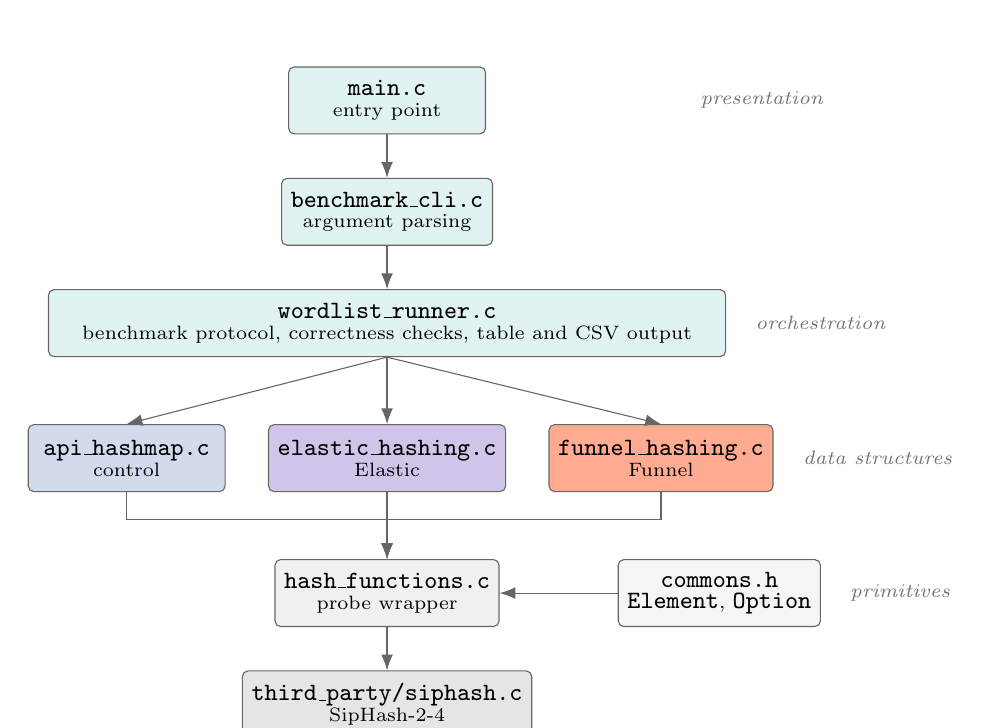
\begin{tikzpicture}[
  node distance=0.55cm and 0.5cm,
  every node/.style={font=\footnotesize},
  mod/.style={draw=black!60,rounded corners=2pt,minimum height=0.85cm,minimum width=2.5cm,
              align=center,fill=white},
  layer/.style={draw=black!25,dashed,rounded corners=4pt,inner sep=0.32cm},
  ar/.style={-{Latex[length=2mm]},draw=black!60}
]
  % layer 1
  \node[mod,fill=accent!12] (main) {\code{main.c}\\[-2pt]\scriptsize entry point};
  \node[mod,fill=accent!12,below=of main] (cli) {\code{benchmark\_cli.c}\\[-2pt]\scriptsize argument parsing};
  \node[mod,fill=accent!12,below=of cli,minimum width=8.6cm] (runner)
       {\code{wordlist\_runner.c}\\[-2pt]\scriptsize benchmark protocol, correctness checks, table and CSV output};
  % layer 3: the three maps
  \node[mod,fill=stdc!25,below left=0.85cm and 2.05cm of runner.south] (api)
       {\code{api\_hashmap.c}\\[-2pt]\scriptsize control};
  \node[mod,fill=T3,below=0.85cm of runner.south] (ela)
       {\code{elastic\_hashing.c}\\[-2pt]\scriptsize Elastic};
  \node[mod,fill=P3,below right=0.85cm and 2.05cm of runner.south] (fun)
       {\code{funnel\_hashing.c}\\[-2pt]\scriptsize Funnel};
  % layer 4
  \node[mod,fill=black!6,below=0.85cm of ela] (hf)
       {\code{hash\_functions.c}\\[-2pt]\scriptsize probe wrapper};
  \node[mod,fill=black!10,below=of hf] (sip)
       {\code{third\_party/siphash.c}\\[-2pt]\scriptsize SipHash-2-4};
  \node[mod,fill=black!4,right=1.5cm of hf,minimum width=2.2cm] (com)
       {\code{commons.h}\\[-2pt]\scriptsize \code{Element}, \code{Option}};
  % arrows
  \draw[ar] (main) -- (cli);
  \draw[ar] (cli) -- (runner);
  \draw[ar] (runner.south) -- (api.north);
  \draw[ar] (runner.south) -- (ela.north);
  \draw[ar] (runner.south) -- (fun.north);
  \draw[ar] (api.south) -- ++(0,-0.35) -| (hf.north);
  \draw[ar] (ela.south) -- (hf.north);
  \draw[ar] (fun.south) -- ++(0,-0.35) -| (hf.north);
  \draw[ar] (hf) -- (sip);
  \draw[ar] (com) -- (hf);
  % layer labels
  \node[anchor=west,font=\scriptsize\itshape,black!55] at ($(main.east)+(2.6,0)$) {presentation};
  \node[anchor=west,font=\scriptsize\itshape,black!55] at ($(runner.east)+(0.25,0)$) {orchestration};
  \node[anchor=west,font=\scriptsize\itshape,black!55] at ($(fun.east)+(0.25,0)$) {data structures};
  \node[anchor=west,font=\scriptsize\itshape,black!55] at ($(com.east)+(0.25,0)$) {primitives};
\end{tikzpicture}
\end{center}
{\captionof{figure}{Block architecture. The three implementations share the same hash
primitive and the same \code{Element} type, but know nothing about each other: this
guarantees that the comparison measures algorithmic differences and not accidental
coupling.}
\label{fig:arch}\par}

\subsection{Data model}

\begin{center}
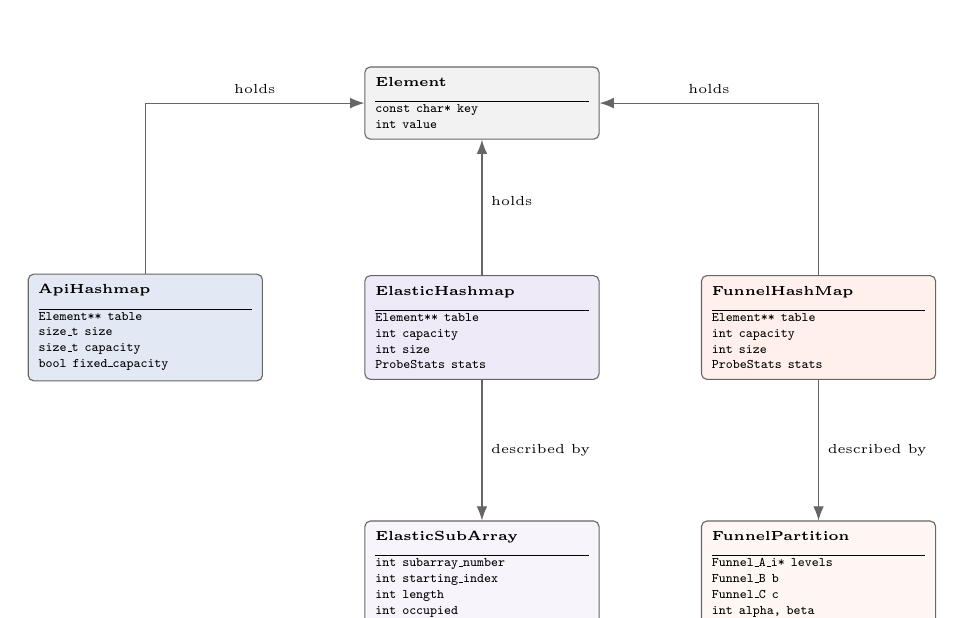
\begin{tikzpicture}[
  scale=0.95, transform shape,
  every node/.style={font=\tiny},
  cls/.style={draw=black!60,rounded corners=2pt,align=left,inner sep=4pt,
              fill=white,text width=2.85cm},
  ar/.style={-{Latex[length=1.8mm]},draw=black!60}
]
\node[cls,fill=black!5] (el) at (0,3.7) {
  \textbf{Element}\\\hrulefill\\[-2pt]
  \texttt{const char* key}\\
  \texttt{int value}
};
\node[cls,fill=stdc!15] (ahm) at (-4.5,0.7) {
  \textbf{ApiHashmap}\\\hrulefill\\[-2pt]
  \texttt{Element** table}\\
  \texttt{size\_t size}\\
  \texttt{size\_t capacity}\\
  \texttt{bool fixed\_capacity}
};
\node[cls,fill=elasticc!15] (ehm) at (0,0.7) {
  \textbf{ElasticHashmap}\\\hrulefill\\[-2pt]
  \texttt{Element** table}\\
  \texttt{int capacity}\\
  \texttt{int size}\\
  \texttt{ProbeStats stats}
};
\node[cls,fill=funnelc!18] (fhm) at (4.5,0.7) {
  \textbf{FunnelHashMap}\\\hrulefill\\[-2pt]
  \texttt{Element** table}\\
  \texttt{int capacity}\\
  \texttt{int size}\\
  \texttt{ProbeStats stats}
};
\node[cls,fill=elasticc!8] (esa) at (0,-2.6) {
  \textbf{ElasticSubArray}\\\hrulefill\\[-2pt]
  \texttt{int subarray\_number}\\
  \texttt{int starting\_index}\\
  \texttt{int length}\\
  \texttt{int occupied}
};
\node[cls,fill=funnelc!10] (fp) at (4.5,-2.6) {
  \textbf{FunnelPartition}\\\hrulefill\\[-2pt]
  \texttt{Funnel\_A\_i* levels}\\
  \texttt{Funnel\_B b}\\
  \texttt{Funnel\_C c}\\
  \texttt{int alpha, beta}
};
\draw[ar] (ahm.north) |- node[above,pos=0.75] {holds} (el.west);
\draw[ar] (ehm.north) -- node[right,pos=0.55] {holds} (el.south);
\draw[ar] (fhm.north) |- node[above,pos=0.75] {holds} (el.east);
\draw[ar] (ehm.south) -- node[right] {described by} (esa.north);
\draw[ar] (fhm.south) -- node[right] {described by} (fp.north);
\end{tikzpicture}
\end{center}
{\captionof{figure}{Main data structures. The partition descriptors
(\code{ElasticSubArray}, \code{FunnelPartition}) own no memory: they contain only indices
and lengths describing ranges of the single \code{table} array owned by the map.}
\label{fig:datamodel}\par}

\subsection{Memory layout}

The most easily misunderstood aspect of both algorithms is that the ``subarrays'' are
logical partitions of a single physical array. Figure~\ref{fig:elastic-layout} makes this
explicit for Elastic Hashing at a toy capacity of $n = 15$.

\begin{center}
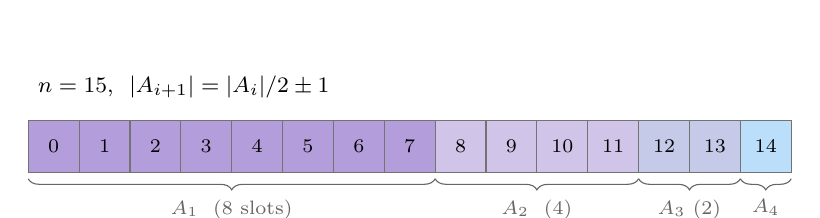
\begin{tikzpicture}[scale=0.95,every node/.style={font=\scriptsize}]
  \foreach \x in {0,...,14} {
    \pgfmathsetmacro{\col}{\x<8 ? 1 : (\x<12 ? 2 : (\x<14 ? 3 : 4))}
    \definecolor{cellcol}{HTML}{B39DDB}
    \ifnum\col=2\definecolor{cellcol}{HTML}{D1C4E9}\fi
    \ifnum\col=3\definecolor{cellcol}{HTML}{C5CAE9}\fi
    \ifnum\col=4\definecolor{cellcol}{HTML}{BBDEFB}\fi
    \draw[fill=cellcol,draw=black!55] (\x*0.68,0) rectangle (\x*0.68+0.68,0.7);
    \node at (\x*0.68+0.34,0.35) {\x};
  }
  \draw[decorate,decoration={brace,amplitude=4pt,mirror},black!60] (0,-0.08) -- (5.44,-0.08)
       node[midway,below=4pt] {$A_1$ \ (8 slots)};
  \draw[decorate,decoration={brace,amplitude=4pt,mirror},black!60] (5.44,-0.08) -- (8.16,-0.08)
       node[midway,below=4pt] {$A_2$ \ (4)};
  \draw[decorate,decoration={brace,amplitude=4pt,mirror},black!60] (8.16,-0.08) -- (9.52,-0.08)
       node[midway,below=4pt] {$A_3$ (2)};
  \draw[decorate,decoration={brace,amplitude=4pt,mirror},black!60] (9.52,-0.08) -- (10.2,-0.08)
       node[midway,below=4pt] {$A_4$};
  \node[anchor=west,font=\footnotesize] at (0,1.15) {$n = 15$, \ $|A_{i+1}| = |A_i|/2 \pm 1$};
\end{tikzpicture}
\end{center}
{\captionof{figure}{The subarrays of Elastic Hashing are index ranges of one physical
array, not separate allocations. At $n = 15$ the four subarrays occupy slots $0..7$, $8..11$,
$12..13$ and $14$.}\label{fig:elastic-layout}\par}

\subsection{State diagram of Elastic Hashing insertion}

Inserting a key during batch $\mathcal{B}_i$ is a state machine driven by the two free-space
fractions $\varepsilon_1 = \varepsilon(A_i)$ and $\varepsilon_2 = \varepsilon(A_{i+1})$,
recomputed \emph{before every insertion}.

\begin{center}
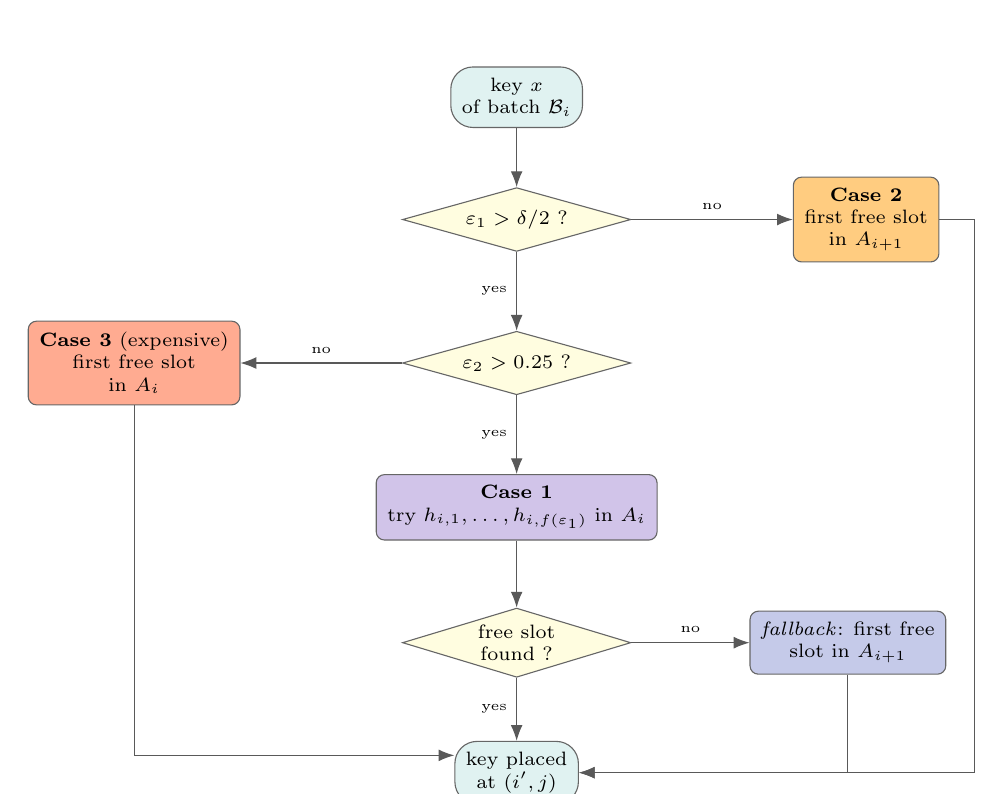
\begin{tikzpicture}[
  node distance=0.75cm and 1.15cm,
  every node/.style={font=\scriptsize},
  st/.style={draw=black!60,rounded corners=3pt,align=center,inner sep=4pt,minimum height=0.8cm,fill=white},
  dec/.style={draw=black!60,diamond,aspect=2.3,align=center,inner sep=0pt,fill=yellow!12,minimum width=2.9cm},
  term/.style={draw=black!60,rounded corners=8pt,align=center,inner sep=4pt,fill=accent!12},
  ar/.style={-{Latex[length=2mm]},draw=black!65}
]
\node[term] (start) {key $x$\\ of batch $\mathcal{B}_i$};
\node[dec,below=of start] (d1) {$\varepsilon_1 > \delta/2$ ?};
\node[dec,below=1.0cm of d1] (d2) {$\varepsilon_2 > 0.25$ ?};
\node[st,fill=T3,below=1.0cm of d2] (c1) {\textbf{Case 1}\\ try
   $h_{i,1},\dots,h_{i,f(\varepsilon_1)}$ in $A_i$};
\node[dec,below=0.85cm of c1] (d3) {free slot\\ found ?};
\node[st,fill=T4,right=1.5cm of d3] (fb) {\emph{fallback}: first free\\
   slot in $A_{i+1}$};
\node[st,fill=P4,right=2.05cm of d1] (c2) {\textbf{Case 2}\\ first free slot\\ in $A_{i+1}$};
\node[st,fill=P3,left=2.05cm of d2] (c3) {\textbf{Case 3} (expensive)\\ first free slot\\ in $A_i$};
\node[term,below=0.8cm of d3] (end) {key placed\\ at $(i',j)$};

\draw[ar] (start) -- (d1);
\draw[ar] (d1) -- node[left,font=\tiny] {yes} (d2);
\draw[ar] (d1) -- node[above,font=\tiny] {no} (c2);
\draw[ar] (d2) -- node[above,font=\tiny] {no} (c3);
\draw[ar] (d2) -- node[left,font=\tiny] {yes} (c1);
\draw[ar] (c1) -- (d3);
\draw[ar] (d3) -- node[above,font=\tiny] {no} (fb);
\draw[ar] (d3) -- node[left,font=\tiny] {yes} (end);
\draw[ar] (fb.south) |- (end.east);
% Case 2 is routed to the right of the fallback box: dropping straight down from c2
% made the vertical segment cut through it.
\draw[ar] (c2.east) -- ++(0.45,0) |- (end.east);
\draw[ar] (c3.south) -- ++(0,-0.3) |- ($(end.west)+(0,0.22)$);
\end{tikzpicture}
\end{center}
{\captionof{figure}{State machine of Elastic Hashing insertion. Cases 2 and 3 are mutually exclusive
within one batch: as soon as $\varepsilon_1 \le \delta/2$ and $\varepsilon_2 \le 0.25$ hold
simultaneously, the batch is over. Lemma 2 guarantees that, with $c$ sufficiently large, the
Case 3 branch is never taken in a batch with probability $1-O(1/|A_i|^2)$.}
\label{fig:elastic-state}\par}

\subsection{Flow diagram of the Elastic Hashing lookup}

\begin{center}
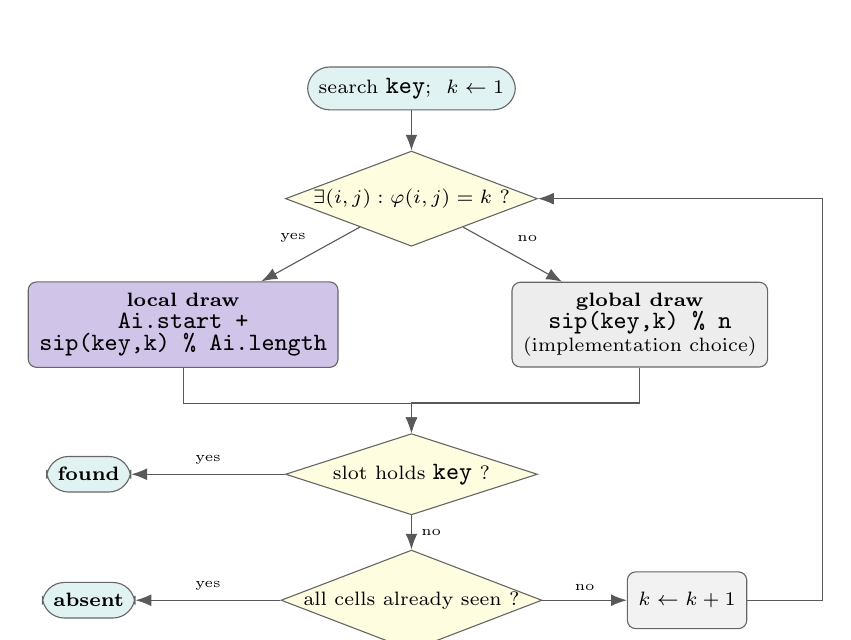
\begin{tikzpicture}[
  every node/.style={font=\scriptsize},
  st/.style={draw=black!60,rounded corners=3pt,align=center,inner sep=4pt,fill=white,minimum height=0.72cm},
  dec/.style={draw=black!60,diamond,aspect=2.6,align=center,inner sep=0pt,fill=yellow!12,minimum width=3.2cm},
  term/.style={draw=black!60,rounded corners=8pt,align=center,inner sep=4pt,fill=accent!12},
  ar/.style={-{Latex[length=2mm]},draw=black!65}
]
\node[term] (s)     at ( 0.0,  0.0) {search \code{key}; \ $k \leftarrow 1$};
\node[dec]  (inv)   at ( 0.0, -1.4) {$\exists (i,j) : \phimap(i,j) = k$ ?};
\node[st,fill=T3] (loc)  at (-2.9, -3.0)
      {\textbf{local draw}\\ \code{Ai.start +}\\ \code{sip(key,k) \% Ai.length}};
\node[st,fill=black!7]     (glob) at ( 2.9, -3.0)
      {\textbf{global draw}\\ \code{sip(key,k) \% n}\\ \scriptsize(implementation choice)};
\node[dec]  (hit)   at ( 0.0, -4.9) {slot holds \code{key} ?};
\node[term] (found) at (-4.1, -4.9) {\textbf{found}};
\node[dec]  (neg)   at ( 0.0, -6.5) {all cells already seen ?};
\node[term] (nf)    at (-4.1, -6.5) {\textbf{absent}};
\node[st,fill=black!5] (inc) at ( 3.5, -6.5) {$k \leftarrow k+1$};

\draw[ar] (s)   -- (inv);
\draw[ar] (inv) -- node[above left,font=\tiny,pos=0.45] {yes} (loc);
\draw[ar] (inv) -- node[above right,font=\tiny,pos=0.45] {no} (glob);
\draw[ar] (loc.south)  -- ++(0,-0.45) -| (hit.north);
\draw[ar] (glob.south) -- ++(0,-0.45) -| (hit.north);
\draw[ar] (hit) -- node[above,font=\tiny] {yes} (found);
\draw[ar] (hit) -- node[right,font=\tiny] {no} (neg);
\draw[ar] (neg) -- node[above,font=\tiny] {yes} (nf);
\draw[ar] (neg) -- node[above,font=\tiny] {no} (inc);
\draw[ar] (inc.east) -- ++(0.95,0) |- (inv.east);
\end{tikzpicture}
\end{center}
{\captionof{figure}{Elastic Hashing lookup. The left branch reproduces exactly the formula
used by insertion and is what guarantees the ``never beyond $\phimap(i,j)$'' invariant. The
right branch covers indices outside the image of $\phimap$ and is an explicit implementation
choice. The negative termination condition is \emph{not} ``empty slot'', because the
algorithm is not greedy, but full coverage of the table, tracked by a bitset.}
\label{fig:elastic-lookup}\par}

\subsection{Measurement protocol}

Every benchmark point follows the same rigid protocol, shown in
Figure~\ref{fig:sequence}. The main requirement is \emph{isolation}: each point builds fresh,
empty maps, does not reuse the previous point's table, and performs no warm-up phase that
would modify the structure being measured.

\begin{center}
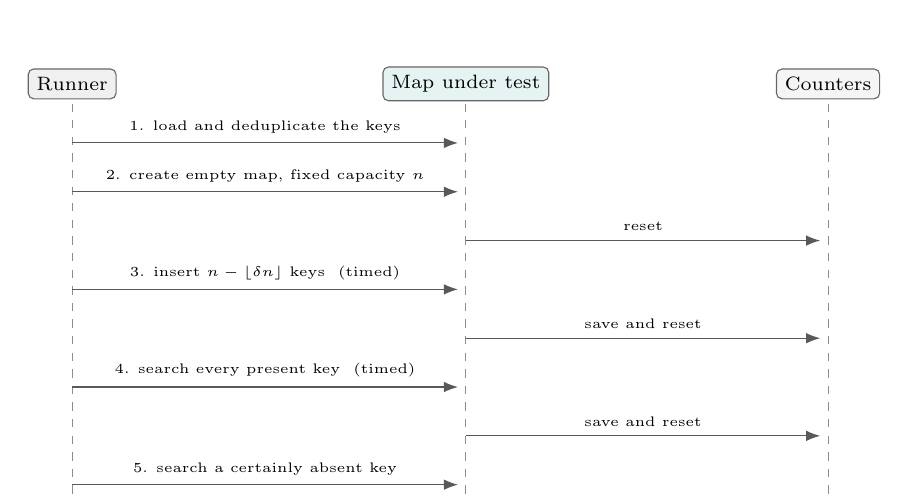
\begin{tikzpicture}[
  every node/.style={font=\scriptsize},
  ar/.style={-{Latex[length=1.8mm]},draw=black!65},
  lifeline/.style={draw=black!45,dashed}
]
\def\ya{0} \def\yb{-0.62} \def\yc{-1.24} \def\yd{-1.86} \def\ye{-2.48}
\def\yf{-3.10} \def\yg{-3.72} \def\yh{-4.34}
% headers
\node[draw=black!60,fill=black!6,rounded corners=2pt,inner sep=3pt] (R) at (0,0.75) {Runner};
\node[draw=black!60,fill=accent!10,rounded corners=2pt,inner sep=3pt] (M) at (5.0,0.75) {Map under test};
\node[draw=black!60,fill=black!4,rounded corners=2pt,inner sep=3pt] (S) at (9.6,0.75) {Counters};
\draw[lifeline] (0,0.5) -- (0,\yh-0.35);
\draw[lifeline] (5.0,0.5) -- (5.0,\yh-0.35);
\draw[lifeline] (9.6,0.5) -- (9.6,\yh-0.35);
% messages
\draw[ar] (0,\ya) -- node[above,font=\tiny] {1. load and deduplicate the keys} (4.9,\ya);
\draw[ar] (0,\yb) -- node[above,font=\tiny] {2. create empty map, fixed capacity $n$} (4.9,\yb);
\draw[ar] (5.0,\yc) -- node[above,font=\tiny] {reset} (9.5,\yc);
\draw[ar] (0,\yd) -- node[above,font=\tiny] {3. insert $n-\lfloor\delta n\rfloor$ keys \ (timed)} (4.9,\yd);
\draw[ar] (5.0,\ye) -- node[above,font=\tiny] {save and reset} (9.5,\ye);
\draw[ar] (0,\yf) -- node[above,font=\tiny] {4. search every present key \ (timed)} (4.9,\yf);
\draw[ar] (5.0,\yg) -- node[above,font=\tiny] {save and reset} (9.5,\yg);
\draw[ar] (0,\yh) -- node[above,font=\tiny] {5. search a certainly absent key} (4.9,\yh);
\end{tikzpicture}
\end{center}
{\captionof{figure}{Protocol of one benchmark point. Counters are saved and reset between the
three phases, so that insertion, positive lookup and negative lookup do not contaminate each
other. The negative lookup is excluded from the timings and probe counts of the other phases
and is reported separately.}
\label{fig:sequence}\par}

A point fails, with explicit diagnostics, if: an
insertion does not succeed; a positive lookup fails to find the key or returns a value other
than the associated one; the negative lookup finds something. The \code{correct} field of the
CSV output records the outcome.

Every run is fully determined by the triple (wordlist, $\delta$,
128-bit SipHash seed). The seed is recorded in every output row; the default value is
\code{000102030405060708090a0b0c0d0e0f}.

\newpage
% =====================================================================
\section{Results}
\label{sec:results}
% =====================================================================

\subsection{Experimental configuration}

\begin{center}
\small
\begin{tabular}{@{}ll@{}}
\toprule
Capacity & $n = 65{,}536$; $\dinv$ is a power of two at every point, as Theorem 1 requires \\
Dataset & \code{english.txt}, 354,297 unique words extracted from English texts \\
Load factors & 87.5\%, 96.875\%, 99.21875\%, 99.609375\% \\
Corresponding $\delta$ & $1/8$, $1/32$, $1/128$, $1/256$ \\
Elastic constant & $c = 100$ \\
SipHash seed & \code{000102030405060708090a0b0c0d0e0f} \\
Build & \code{HashMapsProbes} (\code{-O2}, counters enabled) \\
\bottomrule
\end{tabular}
\end{center}

Each point uses the first $n - \lfloor \delta n \rfloor$ unique words, so the keys of the
least loaded point are a subset of those of the later points. Capacity, seed and wordlist
order stay identical across points.

\subsection{Insertion cost}

\begin{center}
\begin{tikzpicture}
\begin{axis}[
  width=0.94\linewidth, height=6.2cm,
  xlabel={load factor (\%)}, ylabel={average probes per insertion},
  ymode=log, log basis y=10, log ticks with fixed point,
  ytick={3,5,10,20,50,100,200,500,1000,2000,5000,20000},
  minor y tick num=4,
  xmin=-0.35, xmax=3.35,
  grid=both, major grid style={black!12}, minor grid style={black!6},
  legend pos=north west, legend cell align=left,
  legend style={font=\scriptsize,draw=black!30,fill=white,fill opacity=0.92,text opacity=1},
  label style={font=\small}, tick label style={font=\scriptsize},
  xtick={0,1,2,3},
  xticklabels={87.5,96.875,99.219,99.609},
]
\addplot[color=stdc,mark=*,thick]     table[x expr=\coordindex,y=insavg] {wl-standard.dat};
\addplot[color=elasticc,mark=square*,thick] table[x expr=\coordindex,y=insavg] {wl-elastic.dat};
\addplot[color=funnelc,mark=triangle*,thick] table[x expr=\coordindex,y=insavg] {wl-funnel.dat};
\legend{Control (linear probing), Elastic, Funnel}
\end{axis}
\end{tikzpicture}
\end{center}
{\captionof{figure}{Average probes per insertion, $n = 65{,}536$, wordlist
\code{english.txt}. Logarithmic scale.}
\label{fig:ins-avg}\par}

\begin{center}
\small
\begin{tabular}{@{}lrrrrrr@{}}
\toprule
& \multicolumn{2}{c}{\textbf{Control}} & \multicolumn{2}{c}{\textbf{Elastic}}
& \multicolumn{2}{c}{\textbf{Funnel}} \\
\cmidrule(lr){2-3}\cmidrule(lr){4-5}\cmidrule(lr){6-7}
\textbf{Load} & avg & max & avg & max & avg & max \\
\midrule
87.5\,\%      & 4.29  & 363    & \textbf{2.92} & 92  & 17.40 & \textbf{61}  \\
96.875\,\%    & 16.50 & 4,245  & \textbf{4.29} & 395 & 33.29 & \textbf{151} \\
99.21875\,\%  & 45.95 & 11,519 & \textbf{5.57} & 701 & 48.33 & \textbf{295} \\
99.609375\,\% & 61.95 & 18,585 & \textbf{6.17} & 801 & 56.20 & \textbf{544} \\
\bottomrule
\end{tabular}
\end{center}
{\captionof{table}{Insertion probes. The best value in each column group is in bold.}
\label{tab:ins}\par}

This is the clearest result of the whole benchmark.

Elastic Hashing does grow as the table fills, from 2.92 to 6.17 average probes, a factor of
2.1. The comparison is what matters. Over the same range linear probing grows by a factor of
14.4, from 4.29 to 61.95. The point is not that Elastic Hashing is flat, it is that its growth
is far smaller than the control's over the same range. For reference, $\log_2\dinv$ is
$3, 5, 7, 8$ at the four points and $\dinv$ is $8, 32, 128, 256$.

Funnel Hashing wins on the single most expensive insertion of the run. Its worst insertion
grows by a factor of 9 where the control's grows by 51, from 363 to 18,585 probes. That is
what the deterministic $\alpha\beta$ ceiling is there to guarantee, and
Section~\ref{sec:results-insmax} takes it up properly.

Funnel Hashing pays for that with a large constant on the average, since every attempt scans a
whole bucket of $\beta$ slots; it only overtakes the control on the average at the last point.

\subsection{Positive search cost}
\label{sec:results-lookup}

\begin{center}
\begin{tikzpicture}
\begin{axis}[
  width=0.94\linewidth, height=6.2cm,
  xlabel={load factor (\%)}, ylabel={average probes per search},
  ymode=log, log basis y=10, log ticks with fixed point,
  ytick={3,5,10,20,50,100,200,500,1000,2000,5000,20000},
  minor y tick num=4,
  xmin=-0.35, xmax=3.35,
  grid=both, major grid style={black!12}, minor grid style={black!6},
  legend pos=south east, legend cell align=left,
  legend style={font=\scriptsize,draw=black!30,fill=white,fill opacity=0.92,text opacity=1},
  label style={font=\small}, tick label style={font=\scriptsize},
  xtick={0,1,2,3},
  xticklabels={87.5,96.875,99.219,99.609},
]
\addplot[color=stdc,mark=*,thick]     table[x expr=\coordindex,y=lkavg] {wl-standard.dat};
\addplot[color=elasticc,mark=square*,thick] table[x expr=\coordindex,y=lkavg] {wl-elastic.dat};
\addplot[color=funnelc,mark=triangle*,thick] table[x expr=\coordindex,y=lkavg] {wl-funnel.dat};
\legend{Control (linear probing), Elastic, Funnel}
\end{axis}
\end{tikzpicture}
\end{center}
{\captionof{figure}{Average probes per successful search. Elastic Hashing costs between twenty
and eighty times the other two, even though the theory assigns it the best amortized cost.}
\label{fig:lk-avg}\par}

\begin{center}
\small
\begin{tabular}{@{}lrrrrrr@{}}
\toprule
& \multicolumn{2}{c}{\textbf{Control}} & \multicolumn{2}{c}{\textbf{Elastic}}
& \multicolumn{2}{c}{\textbf{Funnel}} \\
\cmidrule(lr){2-3}\cmidrule(lr){4-5}\cmidrule(lr){6-7}
\textbf{Load} & avg & max & avg & max & avg & max \\
\midrule
87.5\,\%      & \textbf{4.29}  & 363     & 345.33    & 61,092   & 17.40 & \textbf{61} \\
96.875\,\%    & \textbf{16.50} & 4,245   & 980.53    & 318,854  & 33.29 & \textbf{151} \\
99.21875\,\%  & \textbf{45.95} & 11,519  & 1,406.22  & 282,627  & 48.33 & \textbf{295} \\
99.609375\,\% & 61.95 & 18,585 & 1,537.47 & 350,895 & \textbf{56.20} & \textbf{544} \\
\bottomrule
\end{tabular}
\end{center}
{\captionof{table}{Successful search probes.}
\label{tab:lk}\par}

Elastic Hashing has the \emph{best}
theoretical search bound, $O(1)$ amortized, yet in measurement it is the worst. The explanation is not an implementation error but the
\emph{constant hidden in the encoding of $\phimap$} (and the current lookup implementation, more on that later). As shown in Figure~\ref{fig:phi2d},
the binary encoding of Lemma 1 starts at $\phimap(1,1) = 13$ and grows rapidly along $j$:
$\phimap(1,2)=57$, $\phimap(1,3)=61$, $\phimap(1,4)=233$, $\phimap(1,8)=937$. 

Since the
search cost \emph{is}, by definition, the index $\phimap(i,j)$, even a very well placed key
(small $j$) pays a few dozen probes, and one placed at the eighth local attempt pays almost
a thousand. None of this violates the bound $\phimap(i,j) \le O(i j^2)$. What is large is the
constant factor hidden inside the $O(\cdot)$.

A second effect makes it worse, and Section~\ref{sec:results-c} quantifies it. Because
$c = 100$ makes the limit $f(\varepsilon)$ so generous that no key ever gives up on $A_i$,
keys keep being placed at higher and higher $j$ inside a nearly saturated subarray, where
$\phimap$ amplifies $j$ quadratically.

For scale, the level-by-level scan of Section~\ref{sec:ijscan}, which does not respect the
cost model, costs 14.44 probes against 351.28 at $\delta = 1/8$ on a generated-key table of
the same size, and its
cost stays around 14 over a 16-fold range of $n$. The gap is the price of measuring the
quantity the theorem is stated over rather than the quantity a fast implementation would
optimize.

None of this says the theorem fails. The cost above is what the lookup pays, whereas Theorem 1
bounds the probe complexity of the placement, and the two are only equal for a greedy scheme.
Section~\ref{sec:results-scaling} measures that quantity instead.

\subsection{Worst single insertion}
\label{sec:results-insmax}

\begin{center}
\begin{tikzpicture}
\begin{axis}[
  width=0.94\linewidth, height=6.0cm,
  xlabel={load factor (\%)}, ylabel={maximum probes per insertion},
  ymode=log, log basis y=10, log ticks with fixed point,
  ytick={3,5,10,20,50,100,200,500,1000,2000,5000,20000},
  minor y tick num=4,
  xmin=-0.35, xmax=3.35,
  grid=both, major grid style={black!12}, minor grid style={black!6},
  legend pos=north west, legend cell align=left,
  legend style={font=\scriptsize,draw=black!30,fill=white,fill opacity=0.92,text opacity=1},
  label style={font=\small}, tick label style={font=\scriptsize},
  xtick={0,1,2,3},
  xticklabels={87.5,96.875,99.219,99.609},
]
\addplot[color=stdc,mark=*,thick]     table[x expr=\coordindex,y=insmax] {wl-standard.dat};
\addplot[color=elasticc,mark=square*,thick] table[x expr=\coordindex,y=insmax] {wl-elastic.dat};
\addplot[color=funnelc,mark=triangle*,thick] table[x expr=\coordindex,y=insmax] {wl-funnel.dat};
\legend{Control (linear probing), Elastic, Funnel}
\end{axis}
\end{tikzpicture}
\end{center}
{\captionof{figure}{Maximum number of probes used by a single insertion. Over the four load
factors the control's maximum grows fifty-fold and Funnel Hashing's nine-fold.}
\label{fig:ins-max}\par}

This section is about \emph{insertion} only, and about the most expensive single insertion of
a run rather than the average one. The distinction matters for Elastic Hashing in particular,
whose insertion and search costs are different quantities.

The gap between Figure~\ref{fig:ins-avg} and Figure~\ref{fig:ins-max} is the most important
experimental message about Funnel Hashing. On average it is more expensive than linear probing
up to very high load factors, but its most expensive single insertion is far cheaper: six
times at the lowest load factor measured, and 28 to 39 times at the other three. For an application with a per-operation latency budget rather than a throughput
target, that is the difference that matters.

It is also worth noting that Funnel Hashing is the only one of the three with a high-probability bound
on the maximum of a run, $O(\log^2\dinv + \log\log n)$, which is why its observed maximum is a
more interpretable diagnostic than that of Elastic Hashing.

At the two highest load factors Funnel Hashing's figures do not depend on the seed at all.
Once the first 34 levels fill completely the worst insertion is $34 \times \beta = 544$
probes, and the totals follow from the partition rather than from the draws. Repeating those
two points with different seeds reproduces them exactly. This is a property of a nearly full funnel, not a sign
that the seed is ignored.

\subsection{Comparison with the theoretical bounds}
\label{sec:results-bounds}

Section~\ref{sec:results-lookup} reported what each lookup costs. The question here is
whether those costs follow the shape each theorem predicts, which is done by dividing the
measurement by the predicted growth and checking whether the ratio is flat across the four
load factors. A flat column means the measurement follows that shape, and its value is one
sample of the hidden constant.

One preliminary decides which columns below are meaningful. What the theorems bound is the
\emph{probe complexity} of a key, meaning its index in its own probe sequence, whereas a
benchmark reports how many probes a search actually performs. 

For the control and
for Funnel Hashing the two coincide. Both are greedy, so their lookup retraces the insertion
sequence and stops at exactly the position the key occupies. For Elastic Hashing they do not,
because the insertion is not greedy and an earlier probe may hit the key's cell by chance, as
Section~\ref{sec:results-scaling} explains at length. The Elastic Hashing column below
therefore uses the mean of $\phimap$ over the keys, which is the theorem's quantity, and not
the measured lookup cost.

\begin{center}
\small
\begin{tabular}{@{}rrrrrrrr@{}}
\toprule
& \multicolumn{2}{c}{\textbf{Control}} & \multicolumn{2}{c}{\textbf{Elastic}}
& \multicolumn{2}{c}{\textbf{Funnel}} & \textbf{Funnel max} \\
\cmidrule(lr){2-3}\cmidrule(lr){4-5}\cmidrule(lr){6-7}\cmidrule(lr){8-8}
$L=\log_2\dinv$ & avg & $\dfrac{\text{avg}}{(1+\dinv)/2}$ & $\overline{\phimap}$ &
$\dfrac{\overline{\phimap}}{L}$ & avg & $\dfrac{\text{avg}}{L}$ &
$\dfrac{\max}{\alpha\beta}$ \\
\midrule
3 & 4.29  & 0.95 & 384.7   & 128.2 & 17.40 & 5.80 & 0.46 \\
5 & 16.50 & 1.00 & 1,774.8 & 355.0 & 33.29 & 6.66 & 0.50 \\
7 & 45.95 & 0.71 & 6,205.6 & 886.5 & 48.33 & 6.90 & 0.55 \\
8 & 61.95 & 0.48 & 9,873.4 & 1,234.2 & 56.20 & 7.03 & 0.81 \\
\bottomrule
\end{tabular}
\end{center}
{\captionof{table}{Measured cost divided by the growth each theorem predicts, at
$n = 65{,}536$. A flat column indicates agreement with that shape. The Elastic Hashing column is
$\overline{\phimap}$, the mean probe complexity over the keys, since that is what Theorem 1
bounds.}
\label{tab:bounds}\par}

Theorem 2 predicts $O(\log\dinv)$ amortized for Funnel Hashing. Dividing by $L$, the ratio
stays between 5.8 and 7.03 across a range in which the average itself more than triples, and
drifts slightly upward within that range.


The next column is a stricter check, because it is against a bound that holds with certainty
rather than in expectation. That ceiling is $\alpha\beta$, a quantity the paper never writes
down. It states the bound as $O(\log^2\dinv)$, and $\alpha\beta$ is what that becomes once
the constants are fixed. Section~\ref{sec:funnel} supplies the reasoning. An insertion tries
the levels $A_1, \dots, A_\alpha$ in order,
and in each one it scans a single bucket of $\beta$ slots, so before it can fall through to
the special array $A_{\alpha+1}$ it has spent at most $\alpha$ levels $\times\ \beta$ slots
$= \alpha\beta$ probes. At $\delta = 1/256$ that is $42 \times 16 = 672$.

The last column of Table~\ref{tab:bounds} divides the observed maximum by $\alpha\beta$. It
stays below 1 at every point, rising from 0.46 to 0.81 as the table fills. 

Theorem 1 predicts $O(1)$ for the amortized expected probe complexity of Elastic Hashing,
which would make $\overline{\phimap}$ flat. It is not: it grows from 385 to 9{,}873, a factor of
26, while $L$ only goes from 3 to 8. Dividing by $L$ does not flatten it either, since that
ratio grows from 128 to 1{,}234.

This is not a contradiction. The constant hidden in that $O(1)$ is around $10^9$ at
$c = 100$, as Section~\ref{sec:results-scaling} works out, so every value in the table sits
about five orders of magnitude below the bound and is free to move within it. 

The bound is not
violated; the cost simply does not \emph{behave} like a constant at these sizes, which is the
practically relevant observation and is traced back to $f(\varepsilon)$, and therefore to $c$.

The control column serves as the harness check. Its ratio to Knuth's classical $(1+\dinv)/2$
lands within 5\,\% at the first two points, then falls to 0.71 and 0.48. Finite $n$ does not
explain the shortfall, since Knuth's exact finite-$n$ formula gives 54.4 and 84.4 at the last
two points against 45.95 and 61.95 measured. Spread does. A single run of linear probing this
close to a full table varies by that much from seed to seed. The harness check therefore
rests on the first two points.

\subsection{Comparison of Elastic Hashing lookup strategies}
\label{sec:results-comparison}

This experiment builds \emph{one} Elastic Hashing table and searches the same keys with the three
strategies discussed in Section~\ref{sec:lookup-elastic}. Since the two blind strategies do
quadratic work, the capacity is reduced to $n = 4096$ ($\delta = 1/8$, 3,584 keys, shared
insertion cost: 2.894 average probes).

\begin{center}
\small
\begin{tabular}{@{}lrrrrr@{}}
\toprule
\textbf{Lookup strategy} & \textbf{avg} & \textbf{max} &
\textbf{within $\phimap$} & \textbf{beyond $\phimap$} & \textbf{negative} \\
\midrule
\code{phi-aware} (adopted)  & \textbf{218.39} & 17,564 & \textbf{100.0\,\%} & \textbf{0} & 32,570 \\
\code{full-table-siphash}   & 2,777.21 & 26,370 & 39.6\,\% & 2,165 & 32,570 \\
\code{modular-double-hash}  & 2,025.45 & 4,096  & 6.4\,\%  & 3,355 & \textbf{4,096} \\
\bottomrule
\end{tabular}
\end{center}
{\captionof{table}{Comparison of the three lookup strategies on the same Elastic Hashing table.
``Within $\phimap$'' is the percentage of keys found no later than their own reconstructed
index $\phimap(i,j)$.}
\label{tab:lookupcmp}\par}

These are the performances of the discarded lookup implementations for Elastic Hashing. Only
the strategy finally adopted keeps the invariant. Every key is found at or before its own
$\phimap(i,j)$, in fact exactly at it in 96\,\% of cases, and earlier in the rest when a
previous probe happens to visit the same cell. 

The two blind strategies overshoot
it for 60\,\% and 94\,\% of keys respectively, and cost roughly ten times more while doing so.

The one thing they buy is negative queries. \code{modular-double-hash} is a full permutation
of the table, so an absent key is settled in exactly $n$ probes instead of the coupon
collector's $n\log n$; it just gives up the positive-query guarantee entirely to get there.
This is the trade-off of Section~\ref{sec:lookup-elastic}.

\subsection{Does Elastic Hashing actually meet its amortized bound?}
\label{sec:results-scaling}

$\phimap(i,j)$ is a ceiling on how hard a key
will be to find, fixed at the moment it is inserted: placing a key at $(i,j)$ is the same act
as deciding that no search for it will ever need more than $\phimap(i,j)$ probes. 

Theorem 1
bounds the average of that ceiling over the keys of a table, in expectation over the hash
draws. Writing $(i_t, j_t)$ for where the $t$-th of the $m = n - \lfloor\delta n\rfloor$ keys
ended up:
\[
    \overline{\phimap} \;=\; \frac{1}{m}\sum_{t=1}^{m} \phimap(i_t, j_t),
    \qquad
    \mathbb{E}\big[\,\overline{\phimap}\,\big] \;=\; O(1) .
\]
The symbol $\overline{\phimap}$ refers to amortized expected probe complexity, which is defined as ``the expected value of the average probe complexity across all of the
keys'', and $\overline{\phimap}$ is exactly that inner average.

A single run yields one $\overline{\phimap}$, that is one sample of the random variable
Theorem 1 bounds. That is enough to show its magnitude and how it moves with $n$ and $\delta$,
though not to estimate the expectation itself.

The lookup's probe count is a different number. A search stops as soon as it meets the key,
and it can meet it early, because an earlier probe may land on the key's cell by chance.
Suppose a key sits at $(1,2)$, so its ceiling is $\phimap(1,2) = 57$; if probe 40 happens to
hit that cell, the search reports 40. 

The count is therefore bounded above by the
probe complexity and is often strictly below it, which makes it a fair measurement of this
implementation but not of the theorem's quantity. 

Getting $\overline{\phimap}$ means working
backwards. Find where each key physically sits, recover the $(i,j)$ that put it there, then
evaluate $\phimap$. That is what \code{measure\_phi\_distribution} does, and it is why both
numbers appear below.

\begin{center}
\begin{tikzpicture}
\begin{axis}[
  width=0.94\linewidth, height=5.5cm,
  xlabel={capacity $n$}, ylabel={probes per search},
  xmode=log, log basis x=2, ymode=log, log basis y=10, log ticks with fixed point,
  xtick={4096,16384,65536,262144,1048576},
  xticklabels={4096,16384,65536,262144,1048576},
  ytick={200,300,500,1000,2000,5000,10000}, minor y tick num=4,
  grid=both, major grid style={black!12}, minor grid style={black!6},
  legend cell align=left, legend columns=2,
  legend style={font=\scriptsize,draw=black!30,at={(0.5,-0.26)},anchor=north,
                /tikz/every even column/.append style={column sep=0.6em}},
  label style={font=\small}, tick label style={font=\scriptsize},
]
\addplot[color=T1,mark=o,thick] table[x=n,y=phi3] {phivsmeasured.dat};
\addlegendentry{$\delta=1/8$: mean $\varphi$ (the bound)}
\addplot[color=T1,dashed,mark=square*,thick] table[x=n,y=meas3] {phivsmeasured.dat};
\addlegendentry{$\delta=1/8$: measured lookup}
\addplot[color=funnelc!80!black,mark=o,thick] table[x=n,y=phi8] {phivsmeasured.dat};
\addlegendentry{$\delta=1/256$: mean $\varphi$ (the bound)}
\addplot[color=funnelc!80!black,dashed,mark=triangle*,thick] table[x=n,y=meas8] {phivsmeasured.dat};
\addlegendentry{$\delta=1/256$: measured lookup}
\end{axis}
\end{tikzpicture}
\end{center}
{\captionof{figure}{Solid lines: the mean of $\phimap(i,j)$ over all keys, which is the
quantity Theorem 1 bounds. Dashed lines: probes actually performed by the $\phimap$-aware
lookup. The solid lines are flat in $n$; the dashed ones rise towards them.}
\label{fig:scaling}\par}

\begin{center}
\small
\begin{tabular}{@{}rrrrr@{}}
\toprule
& \multicolumn{2}{c}{$\delta = 1/8$} & \multicolumn{2}{c}{$\delta = 1/256$} \\
\cmidrule(lr){2-3}\cmidrule(lr){4-5}
$n$ & measured & mean $\phimap$ & measured & mean $\phimap$ \\
\midrule
4,096     & 216.4 & 407.3 & 381.3 & 6,829.9 \\
8,192     & 261.2 & 376.8 & 567.1 & 8,941.5 \\
16,384    & 290.7 & 365.2 & 742.9 & 8,785.3 \\
32,768    & 321.7 & 382.4 & 1,073.2 & 8,137.9 \\
65,536    & 352.1 & 384.7 & 1,473.7 & 9,873.4 \\
131,072   & 370.7 & 379.4 & 2,055.7 & 9,184.3 \\
262,144   & 375.4 & 377.5 & 2,841.7 & 9,111.1 \\
1,048,576 & \textbf{377.3} & \textbf{378.3} & 4,842.0 & --- \\
\bottomrule
\end{tabular}
\end{center}
{\captionof{table}{Measured lookup cost against the model's quantity, over a 256-fold range of
$n$, one seed, $c = 100$. The measured column comes from the benchmark runner
(\code{--csv-load-sweep}); the mean of $\phimap$ from \code{measure\_phi\_distribution}, which
reconstructs each key's placement. The two columns are measured on different key sets, so they
should be compared for shape rather than cell by cell. At $n = 1{,}048{,}576$ the latter was run only for
$\delta = 1/8$, the reconstruction being $O(\text{keys} \times j)$.}
\label{tab:scaling}\par}

The two columns of Table~\ref{tab:scaling} move differently: the ceiling holds its level over
the whole 256-fold range while the measured cost climbs towards it. What does not move at all
is the placement itself. Mean $i$ is 1.72 at every capacity tested and mean $j$ stays between
2.89 and 2.97, so a distribution that does not change with $n$ is what holds the ceiling
flat.

One caveat on reading the last row. The two columns come from different key sets, so the
closeness at the largest capacity shows the same shape rather than a precision. Measured
against the mean of $\phimap$ on \emph{its own} table the pairs run 221.2 / 407.3 at
$n = 4096$ to 351.3 / 384.7 at $n = 65{,}536$, and they close in the same way. 

The gap at small $n$ is accounted for by keys that a probe outside the image of $\phimap$
reaches first, before the walk gets to $\phimap(i,j)$. That share was counted directly, and it
shrinks with capacity: 4.9\,\% of keys at $n = 4096$, then 3.0, 1.6, 1.0 and 0.6\,\% at
$n = 65{,}536$. As the windfall becomes rarer the measured cost rises towards the ceiling
rather than away from it.

So much for $n$. In $\delta$ the picture is the opposite: Table~\ref{tab:bounds} showed the
mean of $\phimap$ growing 26-fold as $\delta$ falls from $1/8$ to $1/256$. Theorem 1's $O(1)$
hides a constant that does not depend on $\delta$ either, so it is worth asking whether that
growth contradicts it. It does not, and the reason is the size of that constant.

The constant can be estimated, and it is worth doing because the number is not obvious. Lemma
3 bounds its Case 1 term by $O(i \cdot \varepsilon \cdot f(\varepsilon)^3)$, substitutes
$f(\varepsilon) \le c\log^2\varepsilon^{-1}$ to get
$O(i \cdot c^3 \cdot \varepsilon \log^6 \varepsilon^{-1})$, and then declares the whole
thing $O(i)$. That last step discards two factors: $c^3$, and the largest value the function
$\varepsilon \log_2^6 \varepsilon^{-1}$ can take.

That function is not small. Writing $\varepsilon = 2^{-u}$ it becomes $2^{-u}u^6$, which is
maximized at $u = 6/\ln 2 \approx 8.66$, that is at $\varepsilon \approx 1/403$, where it
equals $1{,}043$. Multiplying the two discarded factors back in:

\[
    c^3 \cdot \max_\varepsilon \varepsilon \log_2^6 \varepsilon^{-1}
    \;=\; 100^3 \cdot 1{,}043 \;\approx\; 1.0 \times 10^9
    \qquad\text{at } c = 100 .
\]

Two caveats keep this honest. The estimate covers only the factors the proof drops explicitly;
Lemma 3's own $O(\cdot)$ constant is never evaluated in the paper, so $10^9$ is a lower bound
on how loose the envelope is, not the envelope itself. And it bounds rather than predicts: the
largest value measured here, $9{,}873$, sits a factor of $10^5$ under it.

The $\delta$ dependence observed is therefore movement well inside that envelope, not a
breach of it.

What the measurements do show is narrower, and still worth stating. At these sizes the
amortized cost does not \emph{behave} like a constant, and the quantity that moves it is
$f(\varepsilon)$, hence $c$.

That is testable directly. Rebuilding the same table at $n = 16{,}384$ over a range of $c$
gives:

\begin{center}
\small
\begin{tabular}{@{}rrrrrr@{}}
\toprule
$c$ & 1 & 2 & 4 & 16 & 100 \\
\midrule
mean $\phimap$, $\delta = 1/8$   & 94.8 & 115.0 & 174.9 & 341.4 & 365.2 \\
mean $\phimap$, $\delta = 1/256$ & 7{,}569.1 & \textbf{280.2} & 551.4 & 2{,}037.1 & 8{,}785.3 \\
\bottomrule
\end{tabular}
\end{center}
{\captionof{table}{Mean $\phimap$ as a function of $c$, at $n = 16{,}384$.}
\label{tab:phic}\par}

At $\delta = 1/8$ the mean of $\phimap$ falls monotonically with $c$, by a factor of 3.9 from
$c = 100$ to $c = 1$. At $\delta = 1/256$ it falls too, but only down to $c = 2$: at $c = 1$ it
jumps back to 7,569, which is where Case 3 starts firing. The next section measures that
directly, and it is the reason the row is not monotone.

\subsection{Calibrating the constant \texorpdfstring{$c$}{c}}
\label{sec:results-c}

The paper requires $c$ to be ``sufficiently large'' without fixing it. This experiment
($n = 16{,}384$, $\delta = 1/8$, 14,336 keys) measures eight values.

\begin{center}
\begin{tikzpicture}
\begin{axis}[
  width=0.68\linewidth, height=5.4cm,
  xlabel={constant $c$}, ylabel={average probes per search},
  xmode=log, log basis x=10,
  grid=both, major grid style={black!12}, minor grid style={black!6},
  label style={font=\small}, tick label style={font=\scriptsize},
  axis y line*=left,
  xtick={0.25,1,4,16,100}, xticklabels={0.25,1,4,16,100},
]
\addplot[color=elasticc,mark=square*,thick] table[x=c,y=lkavg] {csweep.dat};
\label{plt:lk}
\end{axis}
\begin{axis}[
  width=0.68\linewidth, height=5.4cm,
  axis y line*=right, axis x line=none,
  ylabel={insertions in Case 3}, xmode=log,
  ylabel style={font=\small}, tick label style={font=\scriptsize},
  ylabel near ticks,
]
\addlegendimage{/pgfplots/refstyle=plt:lk}\addlegendentry{\scriptsize search (left)}
\addplot[color=red!75,mark=o,thick,dashed] table[x=c,y=case3] {csweep.dat};
\addlegendentry{\scriptsize Case 3 (right)}
\end{axis}
\end{tikzpicture}
\end{center}
{\captionof{figure}{Effect of the constant $c$ at $n = 16{,}384$, $\delta = 1/8$. The search
curve has a clear minimum around $c = 1$; the expensive Case 3 appears only for $c < 1$.}
\label{fig:csweep}\par}

\begin{center}
\small
\begin{tabular}{@{}rrrrrr@{}}
\toprule
$c$ & \textbf{ins.\ avg} & \textbf{search avg} & \textbf{Case 1} &
\textbf{fallbacks} & \textbf{Case 3} \\
\midrule
0.25 & 2.94 & 242.86 & 6,786 & 5,476 & 1,406 \\
0.50 & 2.89 & 166.19 & 7,713 & 5,446 & 479 \\
1.00 & 2.90 & \textbf{90.44} & 7,778 & 5,029 & \textbf{0} \\
2.00 & 2.91 & 115.56 & 4,767 & 1,985 & 0 \\
4.00 & 2.89 & 163.07 & 3,402 & 598 & 0 \\
8.00 & 2.92 & 230.55 & 2,955 & 140 & 0 \\
16.00 & 2.92 & 285.62 & 2,825 & 9 & 0 \\
100.00 & 2.91 & 290.68 & 2,816 & \textbf{0} & 0 \\
\bottomrule
\end{tabular}
\end{center}
{\captionof{table}{Sweep of the Elastic constant $c$.}
\label{tab:csweep}\par}

Three things come out of the sweep.

\begin{enumerate}\itemsep0.6em
  \item \emph{Insertion cost is untouched.} It stays near 2.9 probes for every value tested.
        The parameter governs \emph{where} keys are placed, not what it costs to place them.
  \item \emph{Search cost has a minimum near $c = 1$}, a factor of 3 below $c = 100$. The
        \emph{fallbacks} column explains it: at $c = 1$ most keys give up on $A_i$ early and
        find room at small $j$ in $A_{i+1}$, while at $c = 100$ none give up and all of them
        stay in a saturated $A_i$ at high $j$.
  \item \emph{Below $c = 1$ the cost rises again}, because the expensive Case 3 starts firing.
        This is the phenomenon Lemma 2 excludes when $c$ is large enough.
\end{enumerate}

That minimum is not a recommendation, for two separate reasons.

\begin{enumerate}\itemsep0.6em
  \item \emph{It sits outside the theorem.} The proof of Lemma 2 needs
        $\frac{m}{c}\cdot O(1) < 0.01\,m$, that is $c > 100\,C$ for a constant $C$ the proof
        never evaluates. No smallest admissible $c$ follows from the paper, but the order of
        magnitude does: a hundred rather than one. At $c = 1$ the guarantee that Case 3 does
        not occur no longer applies.
  \item \emph{The safe threshold moves with $\delta$.} Repeating the sweep at
        $\delta = 1/256$, Case 3 still fires 73 times at $c = 1$ and only vanishes from
        $c = 2$, which is also what produces the anomalous mean $\phimap$ of 7,569 in
        Table~\ref{tab:phic}. So $c = 1$ is optimal at one load factor and outside Lemma 2's
        guarantee at another, with no way to know from the paper where the boundary sits.
\end{enumerate}

The benchmarks therefore run at $c = 100$ throughout, and $c = 1$ is reported as an
observation about the finite regime rather than as advice. What $c$ buys is in any case
finite-size only: it shifts the distribution of $j$ values and so the arithmetic size of
$\phimap(i,j)$, which is cheap only for the concrete encoding of Lemma~1.
Section~\ref{sec:results-lookup} shows that encoding dominates the finite search cost whatever
$c$ is set to.

\subsection{Negative queries}
\label{sec:results-negative}

\begin{center}
\small
\begin{tabular}{@{}lrrrr@{}}
\toprule
\textbf{Load factor} & 87.5\,\% & 96.875\,\% & 99.21875\,\% & 99.609375\,\% \\
\midrule
Control & 14 & 96 & 1,323 & 1,506 \\
Funnel Hashing & 52 & 147 & 288 & 545 \\
Elastic Hashing & 787,563 & 787,563 & 787,563 & 787,563 \\
\midrule
$(i,j)$ scan & 68 & 357 & 1,897 & 3,684 \\
\bottomrule
\end{tabular}
\end{center}
{\captionof{table}{Probes for a single absent-key search, $n = 65{,}536$. The last row is the
level-by-level scan of Section~\ref{sec:ijscan} run on the same Elastic Hashing table, kept
below the rule because it does not follow the paper's cost model. It is the average over
1{,}000 absent keys, where the other three rows are a single key, and it is measured on
generated keys rather than on the wordlist.}
\label{tab:neg}\par}

The Elastic Hashing figure is kept separate from the others because it measures an
\emph{implementation extension} and not a result of the paper: the theorems concern present
keys only. Two things about that number line up with Section~\ref{sec:lookup-elastic}.

It does not move with the load factor at all, and in fact cannot: the walk stops on full
coverage of the table, so for a given key and seed the number of draws needed is fixed by $n$
alone and is independent of what the table contains.

The second is the size of the number. Covering $n$ cells by sampling with replacement is the
coupon collector's problem, whose expected cost is $n H_n \approx 764{,}646$, and the measured
787{,}563 sits 3\,\% above it. The agreement is looser than 3\,\% makes it sound. That
distribution has a standard deviation of about 84{,}000 at this $n$, or 11\,\% of its mean,
so a single run landing 3\,\% from the mean is a quarter of a standard deviation out. What
the measurement establishes is the order of magnitude, and the absence of any gross departure
from uniform sampling. One run cannot establish more.

Funnel Hashing, being greedy, settles a negative query at the same order of cost as a positive
one, and at the two highest load factors it cost less than the control's single query in this
run.

The last row is the clearest practical result in the report. The scan gives up on a level at
its first empty slot, so an absent key costs it one early exit per level, and it settles the
query between 210 and 11{,}600 times more cheaply than the cost model's own walk. The
$\phimap$-aware lookup has no stopping rule at all, which is why its cost does not even depend
on $\delta$. Negative queries are outside what the theorems bound, and this is what insisting
on their cost model costs anyway.

\newpage

% =====================================================================
\section{Scope: what this project adds, and what already existed}
\label{sec:scope}
% =====================================================================

\subsection{Where the paper stops}

Section~\ref{sec:related} placed the paper in its literature; what matters here is where it
stops, because that boundary is what an implementation has to cross. Three things are left
open, and each one has already appeared in this report at the point where it had to be
resolved.

The probe complexity of a key is defined as the index at which the key was \emph{placed} in
its own probe sequence, a property of the placement rather than of any search routine, so the
paper owes no search algorithm and for Elastic Hashing gives none
(Section~\ref{sec:lookup-elastic}). No constant is ever fixed: $c$ is required only to be
``sufficiently large'', and the constants hidden by the $O(\cdot)$ notation are never
estimated (Sections~\ref{sec:results-c} and~\ref{sec:results-scaling}). And every bound
concerns keys that are present. Negative queries are discussed only for greedy schemes, where
the paper observes they cost the same as an insertion; for Elastic Hashing nothing is said
(Section~\ref{sec:results-negative}).

These are not defects. They are the normal boundary of a theoretical result.

\subsection{What already existed}

Section~\ref{sec:related} lists the independent implementations and the clauses where they
depart from the paper. Two things can be added now that the measurements exist.

The first is that on search they are faster than the implementation described here, and by a
wide margin: on a generated-key table at $n = 65{,}536$ and $\delta = 1/8$ the level-by-level
scan answers a positive query in 14.44 probes against 351.28, and a negative one in 68 against
787{,}563. It is not a like-for-like comparison, since the two procedures count different
things, but no reading of the numbers makes this implementation the faster one.

The second is a defect that only shows up under measurement. The scan in \cite{optopenhash}
caps the local attempt $j$ at the level length, while this project's insertion is unbounded
in $j$ and samples with replacement, so a key can be placed past that cap and become unreachable:
reproducing the bound on our table at $\delta = 1/256$ loses 3 keys out of 65{,}280. Raising
the cap to $8|A_i|$ recovers all of them for 1.2\,\% more probes. It appears only at high
load factors, which is presumably why it has gone unnoticed.

\subsection{What this project adds}

Four things, none of which is speed.

\begin{enumerate}\itemsep0.9em

  \item \emph{Measurement of the quantity the theorems are stated over.} The published
        benchmarks that could be inspected compare wall-clock time against the language's
        built-in hash map \cite{karpeles}, a reasonable engineering question but a different
        one; no published measurement of probe complexity against load factor was found.

  \item \emph{Conformance}, checked mechanically rather than by reading: a separate test
        suite walks the specification clause by clause and asserts each one on the structures
        the code actually builds. Writing those assertions is what turned up two places where
        the paper's text is not literally implementable, the typo in Lemma 1's construction of
        $\phimap$ and the inequality $\sum_{j>i}|A_j| > 2.5|A_i|$ that does not follow from
        the recurrence once the terms reach single digits.

  \item \emph{The negative-query result} of Section~\ref{sec:results-negative}, the finding
        with the clearest practical consequence, and one for which we found no published
        measurement.

  \item \emph{An executable search consistent with the paper's cost model.} Its value is
        narrower than it may look, so it is worth stating precisely. Verifying the theorem
        does not require it: probe complexity is a property of the placement and can be
        computed by instrumenting the insertion alone. What the search establishes is that
        the cost model is \emph{realizable}, that some procedure a real query can run never
        exceeds $\phimap(i,j)$. Without it, $\phimap$ would be an accounting device, and one
        could fairly ask whether it bounds anything a query can actually do.

\end{enumerate}
% =====================================================================
\section{Conclusions}
\label{sec:conclusions}
% =====================================================================

Both schemes were implemented in C on string keys, together with a linear-probing control
table and a harness that counts the physical probes of every operation exactly.

Three measurements carry the report:

\begin{enumerate}\itemsep0.9em

  \item \emph{Elastic Hashing costs the least to fill.} At 99.6\,\% occupancy an insertion
        averages 6.17 probes against 61.95 for linear probing, and the gap widens as the table
        fills: across the four load factors measured its cost grows by a factor of 2.1 while
        the control's grows by 14.4.

  \item \emph{Funnel Hashing bounds the most expensive single insertion.} The worst insertion
        of an entire run costs it 544 probes where the control needs 18{,}585, and it stayed
        under the deterministic ceiling $\alpha\beta$ at every point measured. That is the
        property its theorem is built to deliver, and the one that matters when a bound on the
        single worst operation is worth more than a good average.

  \item \emph{Elastic Hashing's best theoretical property is invisible at these sizes.} The
        $O(1)$ amortized search cost ought to make it the fastest of the three; a search
        instead averages 345 probes at $\delta = 1/8$, where linear probing needs 4.29.

        Neither the implementation nor the theorem is at fault. A search is charged the
        integer $\phimap(i,j)$, and that encoding already asks 13 probes for the best
        placement a key can get and 114 for the second attempt in the second subarray. Whatever
        constant hides inside the $O(\cdot)$, it is large enough to swamp the asymptotic
        advantage at every capacity measured here, and an analysis stated up to constants could
        not have shown that. This is the finding that most needed an implementation to become
        visible.

\end{enumerate}

One result reaches past the paper. Followed literally, its cost model leaves a non-greedy
table no way to stop early on an absent key, so a negative query has to cover the whole array:
787{,}563 probes measured, against 68 for the level-by-level scan the published
implementations use. Any workload with absent keys therefore has to search an Elastic Hashing
table by a procedure the cost model does not describe. That gap does not appear to have been
quantified anywhere, and it is the result here with the most direct consequence for anyone
building on the scheme.

Two limits are worth stating plainly, because they bound what the numbers above are allowed to
mean. Every point comes from a single seed, so the measurements show shape and magnitude but
cannot estimate the expectations the theorems are actually stated over; that would need a
multi-seed run. And a probe count says nothing about what these structures cost to run, which
would need a timing benchmark against CPU cycles. Probes came first here only because they are
the quantity the theorems bound and are independent of machine and language.

If the finite search cost of Elastic Hashing were the target, the measurements point at the
encoding of $\phimap$ rather than at any algorithmic choice. A cheaper injection, still
satisfying $\phimap(i,j) \le O(i j^2)$ but with a smaller multiplicative constant, would move
it without stepping outside Theorem 1. Lowering $c$ moves it too, but only by leaving the
theorem's hypotheses behind (Section~\ref{sec:results-c}).

% =====================================================================
\begin{thebibliography}{99}
\small
\setlength{\itemsep}{0.25em}
\setlength{\parskip}{0pt}
\bibitem{paper} M.~Farach-Colton, A.~Krapivin, W.~Kuszmaul.
\emph{Optimal Bounds for Open Addressing Without Reordering}.
arXiv:2501.02305v2 [cs.DS], 2025.

\bibitem{yao1985} A.~C.~Yao. \emph{Uniform Hashing is Optimal}.
Journal of the ACM, 32(3):687--693, 1985.

\bibitem{ullman1972} J.~D.~Ullman. \emph{A Note on the Efficiency of Hashing Functions}.
Journal of the ACM, 19(3):569--575, 1972.

\bibitem{knuth1963} D.~E.~Knuth. \emph{Notes on ``Open'' Addressing}.
Unpublished memorandum, 1963.

\bibitem{knuth1998} D.~E.~Knuth. \emph{The Art of Computer Programming, Volume III:
Sorting and Searching}. Addison-Wesley, 2nd edition, 1998.

\bibitem{brent1973} R.~P.~Brent. \emph{Reducing the Retrieval Time of Scatter Storage
Techniques}. Communications of the ACM, 16(2):105--109, 1973.

\bibitem{gonnet1979} G.~H.~Gonnet, J.~I.~Munro. \emph{Efficient Ordering of Hash Tables}.
SIAM Journal on Computing, 8(3):463--478, 1979.

\bibitem{tinypointers} M.~A.~Bender, A.~Conway, M.~Farach-Colton, W.~Kuszmaul,
G.~Tagliavini. \emph{Tiny Pointers}. Proc.\ ACM-SIAM SODA, pp.~477--508, 2023.

\bibitem{berenbrink2000} P.~Berenbrink, A.~Czumaj, A.~Steger, B.~V\"ocking.
\emph{Balanced Allocations: The Heavily Loaded Case}. Proc.\ ACM STOC, pp.~745--754, 2000.

\bibitem{optopenhash} \emph{optopenhash}: Python implementation of the paper's hash
tables. \url{https://github.com/sternma/optopenhash}

\bibitem{jorgik} \emph{elastic-hash}: Python implementation of Elastic and Funnel Hashing.
\url{https://github.com/jorgik1/elastic-hash}

\bibitem{karpeles} \emph{elastichash}: Go implementation with benchmarks against the
built-in map. \url{https://github.com/KarpelesLab/elastichash}

\bibitem{bdragon} \emph{elastic-funnel-hash}: Go proof of concept.
\url{https://github.com/bdragon300/elastic-funnel-hash}

\bibitem{ascv} \emph{elastic-funnel-hashing}: C++ implementation.
\url{https://github.com/ascv0228/elastic-funnel-hashing}

\bibitem{siphash} J.-P.~Aumasson, D.~J.~Bernstein. \emph{SipHash: A Fast Short-Input PRF}.
Proc.\ INDOCRYPT, pp.~489--508, 2012.
\end{thebibliography}

\appendix
\newpage
% =====================================================================
\section{User manual}
\label{app:manual}
% =====================================================================

\subsection{Building}

\begin{lstlisting}
cmake -S . -B cmake-build-release -DCMAKE_BUILD_TYPE=Release
cmake --build cmake-build-release --target HashMaps HashMapsProbes -j
\end{lstlisting}

Two executables are produced, running the same algorithms and the same correctness checks:

\begin{itemize}
  \item \code{HashMaps}: no counters, to be used for timing measurements;
  \item \code{HashMapsProbes}: defines \code{HASHMAP\_COUNT\_PROBES=1} and reports probes
        and diagnostics.
\end{itemize}

\emph{Timings from the two builds must not be compared directly}, because the instrumented
one adds counter writes. In CLion it is enough to reload CMake, select one of the two
targets and put the arguments in the \emph{Program arguments} field.

\subsection{Modes}

Commands accept the names \code{standard}, \code{elastic}, \code{funnel},
\code{both} (control + Elastic), \code{funnel-control} (control + Funnel) and
\code{all} (all three).

\subsection{Main commands}

The full command reference, including every mode, every \code{--csv-} variant and the format
of each output column, is in the repository \code{README}. Reproducing the measurements of
Section~\ref{sec:results} needs only one script:

\begin{lstlisting}
./reproduce_benchmarks.sh [output_dir] [wordlist]
\end{lstlisting}

It rebuilds both targets, echoes each command before running it, writes the CSV files and
prints a summary table that can be compared line by line against Tables~\ref{tab:ins},
\ref{tab:lk} and \ref{tab:bounds}. Every run is determined by the triple (wordlist, $\delta$,
128-bit seed); the seed appears in every output row and defaults to
\code{000102030405060708090a0b0c0d0e0f}.

Two operational points are worth stating here rather than in the \code{README}, because they
affect how the numbers in this report should be read. Keys are split on \code{isspace} and are
\emph{not} normalized, so \code{word}, \code{Word} and \code{word,} count as three distinct
keys. 

If Funnel Hashing's integer partition does not exist for a given $(n,\delta)$, that point is
skipped with a message on standard error and produces no row, rather than producing a wrong
number.
\end{document}
